\chapter{Resultados}\label{chp-07}

Finalmente, aunando todo el desarrollo expuesto en los capítulos precedentes se expone en este
capítulo el resultado del trabajo y su conversión del campo teórico a la práctica.

\section{Placas}

Siguiendo con el diseño electrónico se han fabricado las placas electrónicas necesarias para el proyecto.
En la figura \ref{fig:placafondo} y en la figura \ref{fig:placatapa} se muestran las placas con 
sus pistas y sus componentes soldados.

\begin{figure}[hbtp]%  
    \centering 
        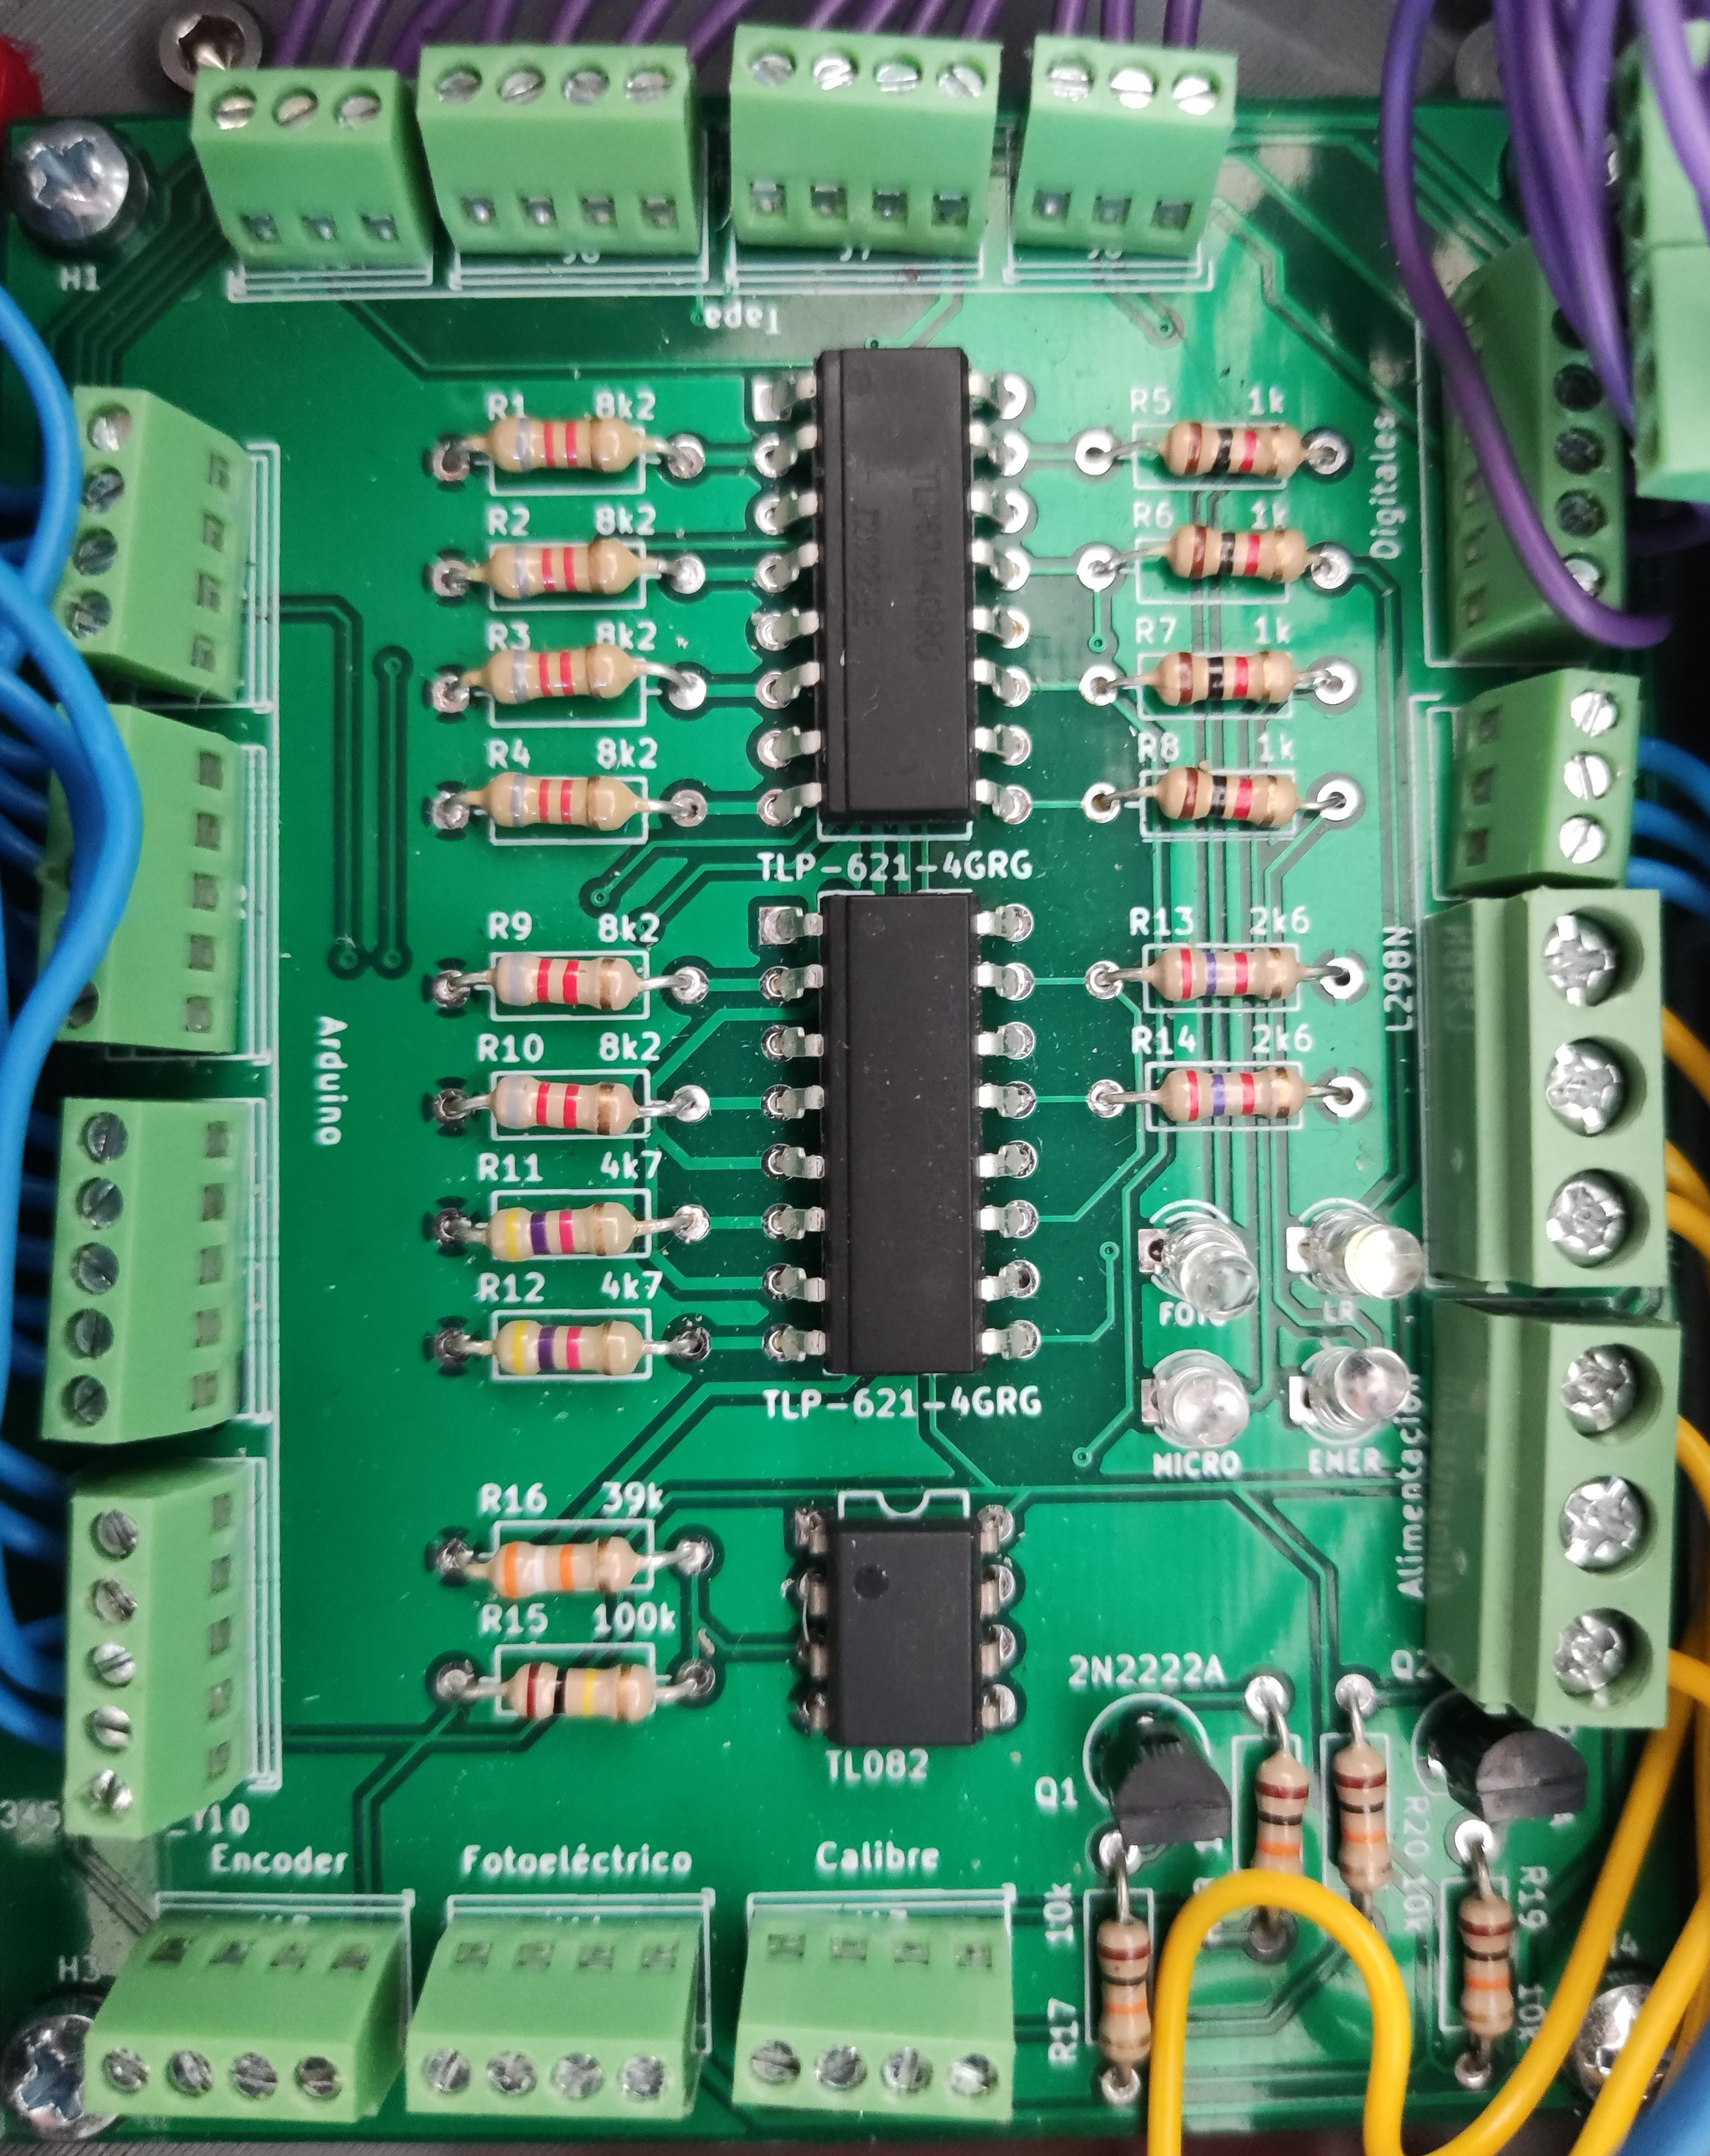
\includegraphics[width=0.4\textwidth]{07-resultados/placafondo.jpg}
    \caption{}
    \label{fig:placafondo} 
\end{figure}

\begin{figure}[hbtp]%  
    \centering 
        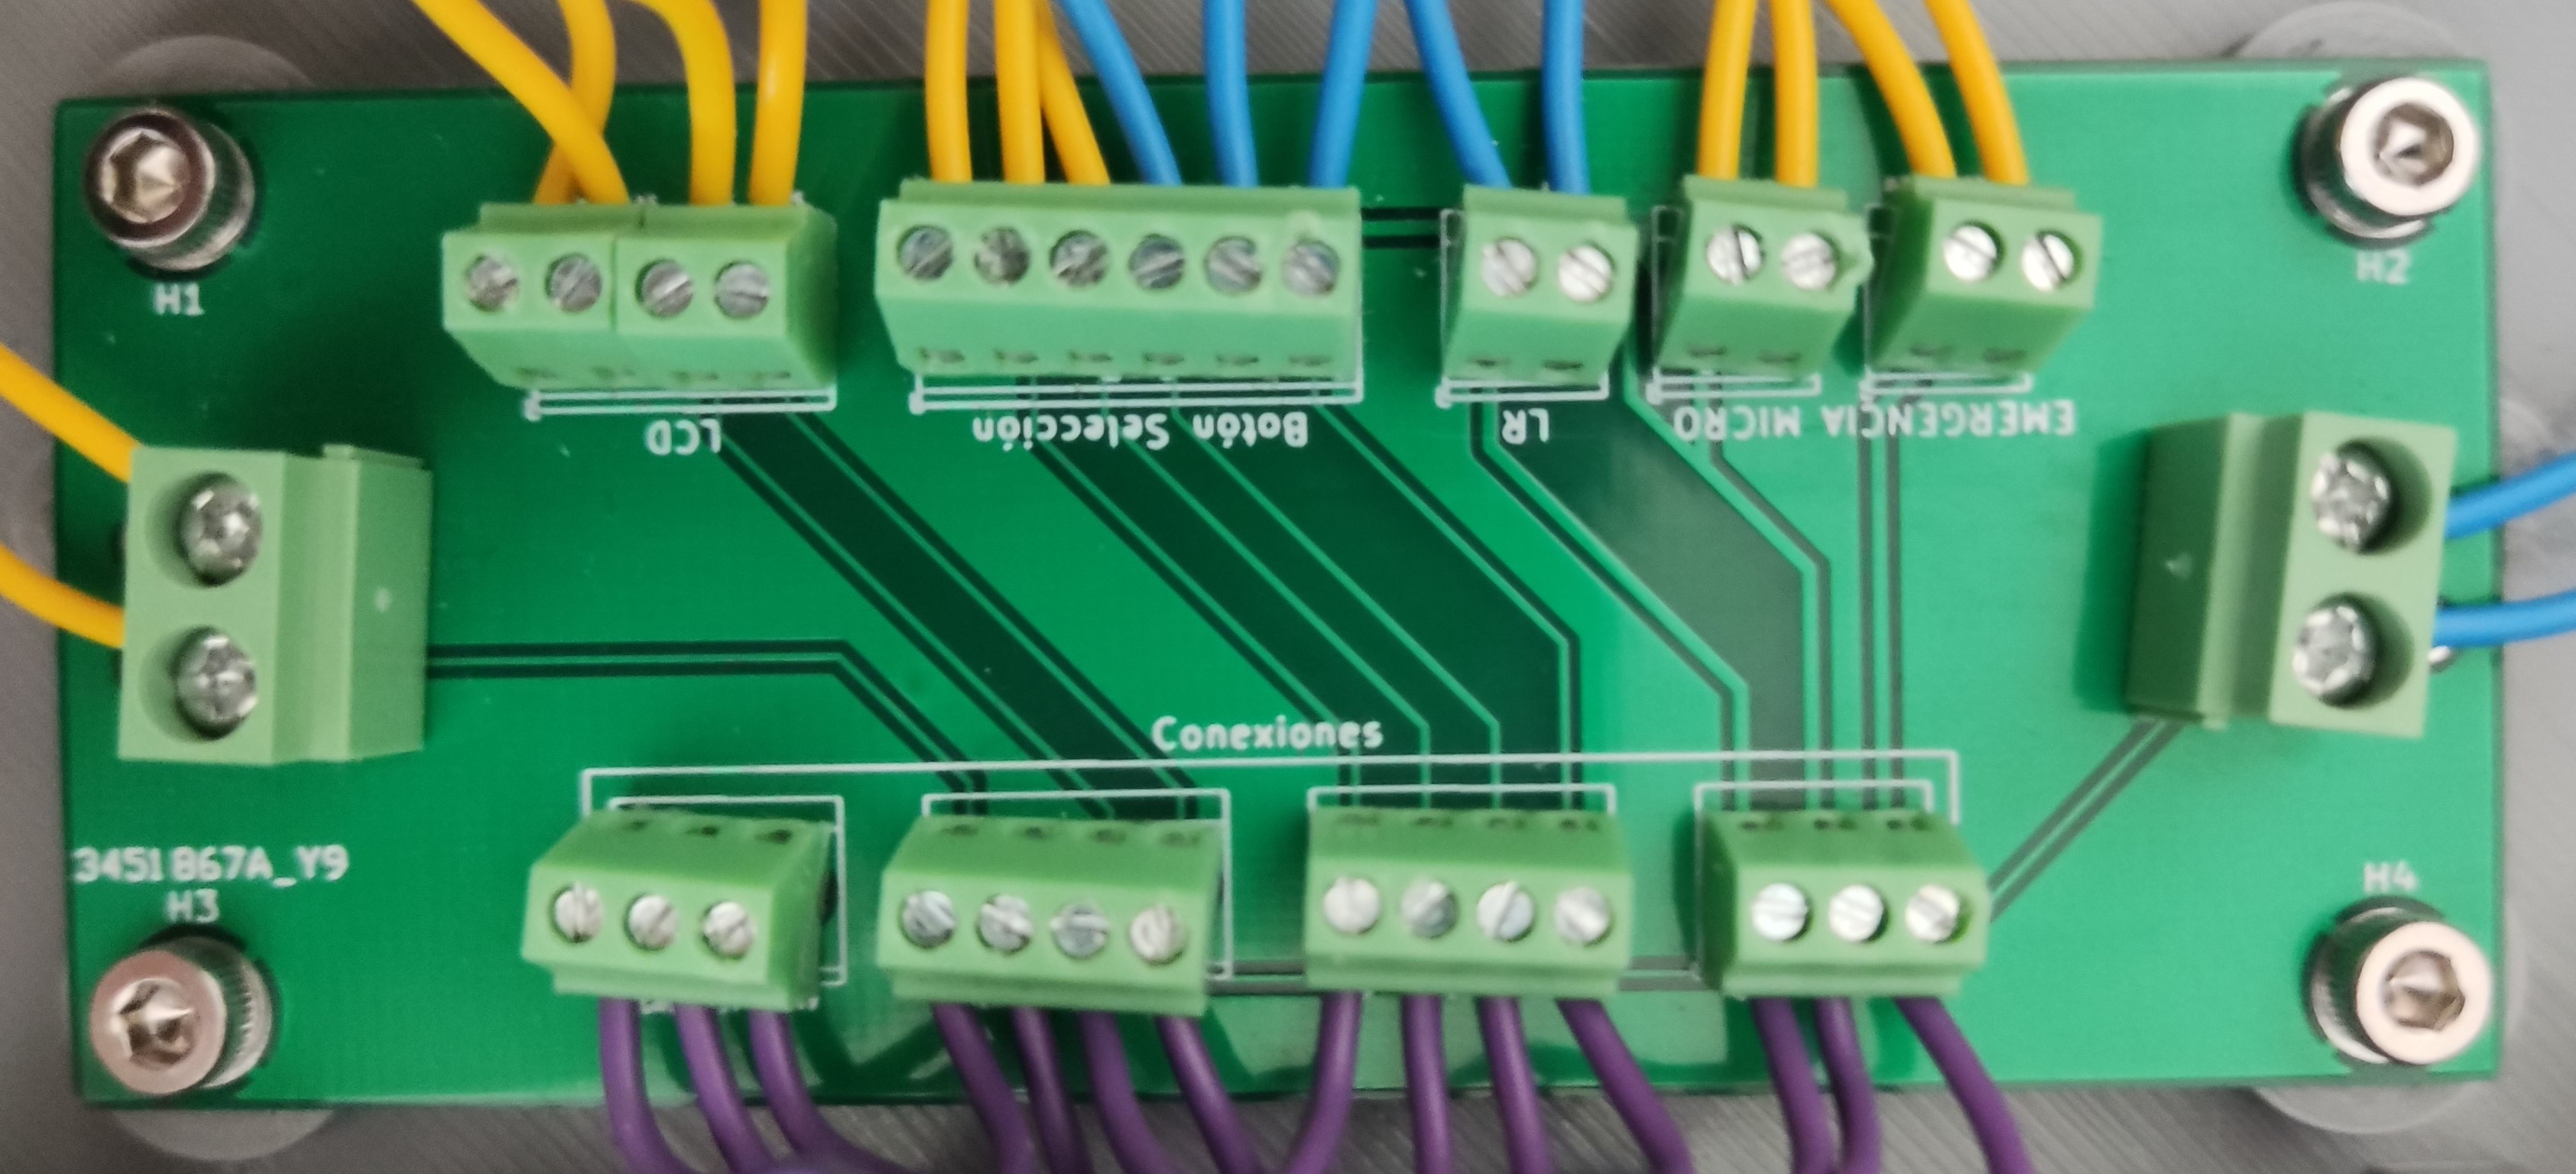
\includegraphics[width=0.75\textwidth]{07-resultados/placatapa.jpg}
    \caption{}
    \label{fig:placatapa} 
\end{figure}

\section{Caja}

La caja se ha impreso en 3D la caja y se ha ensamblado. En la figura \ref{fig:cajaexterior}
se muestra en perspectiva la caja con todos sus elementos unidos, tanto la base como la tapa. 
Además se muestra la interfaz humano-máquina al completo.

\begin{figure}[hbtp]%  
    \centering 
        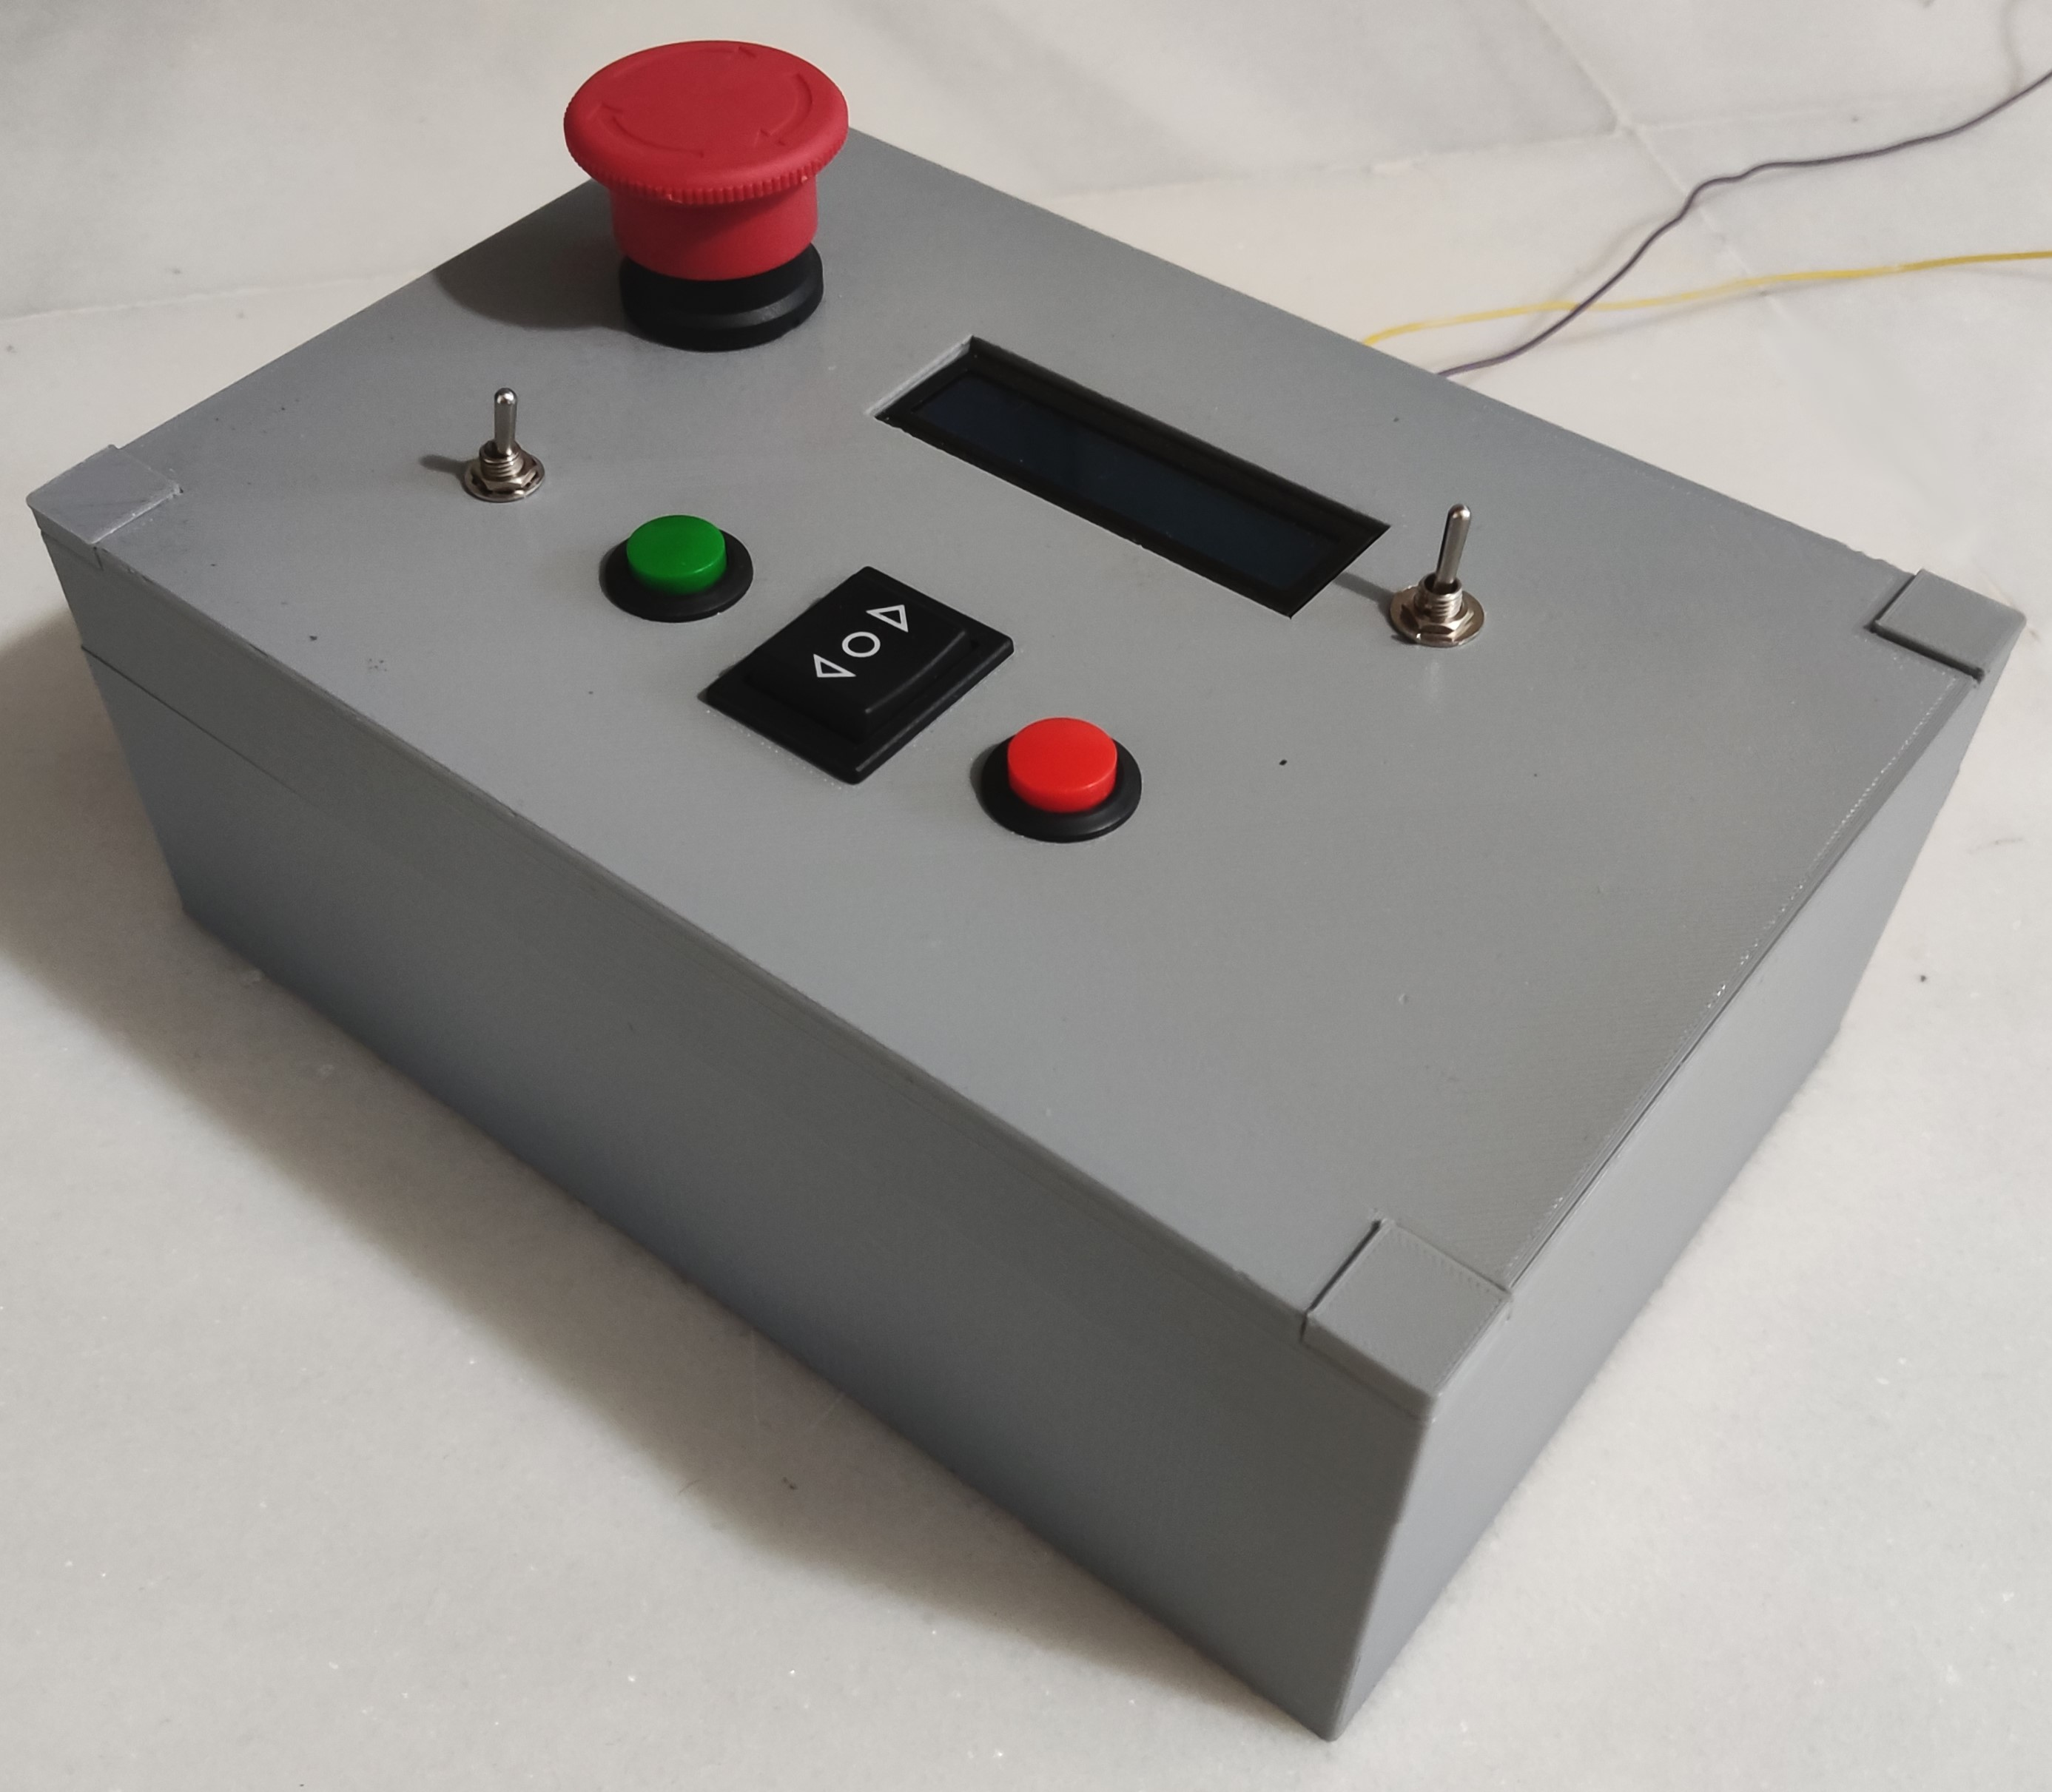
\includegraphics[width=0.75\textwidth]{07-resultados/cajaexterior.jpg}
    \caption{}
    \label{fig:cajaexterior} 
\end{figure}

En la figura \ref{fig:cajatrasero} se muestra la parte trasera de la caja, donde se encuentra
el orificio donde se introducen los cables, el conector Ethernet y los pines digitales.

\begin{figure}[hbtp]%  
    \centering 
        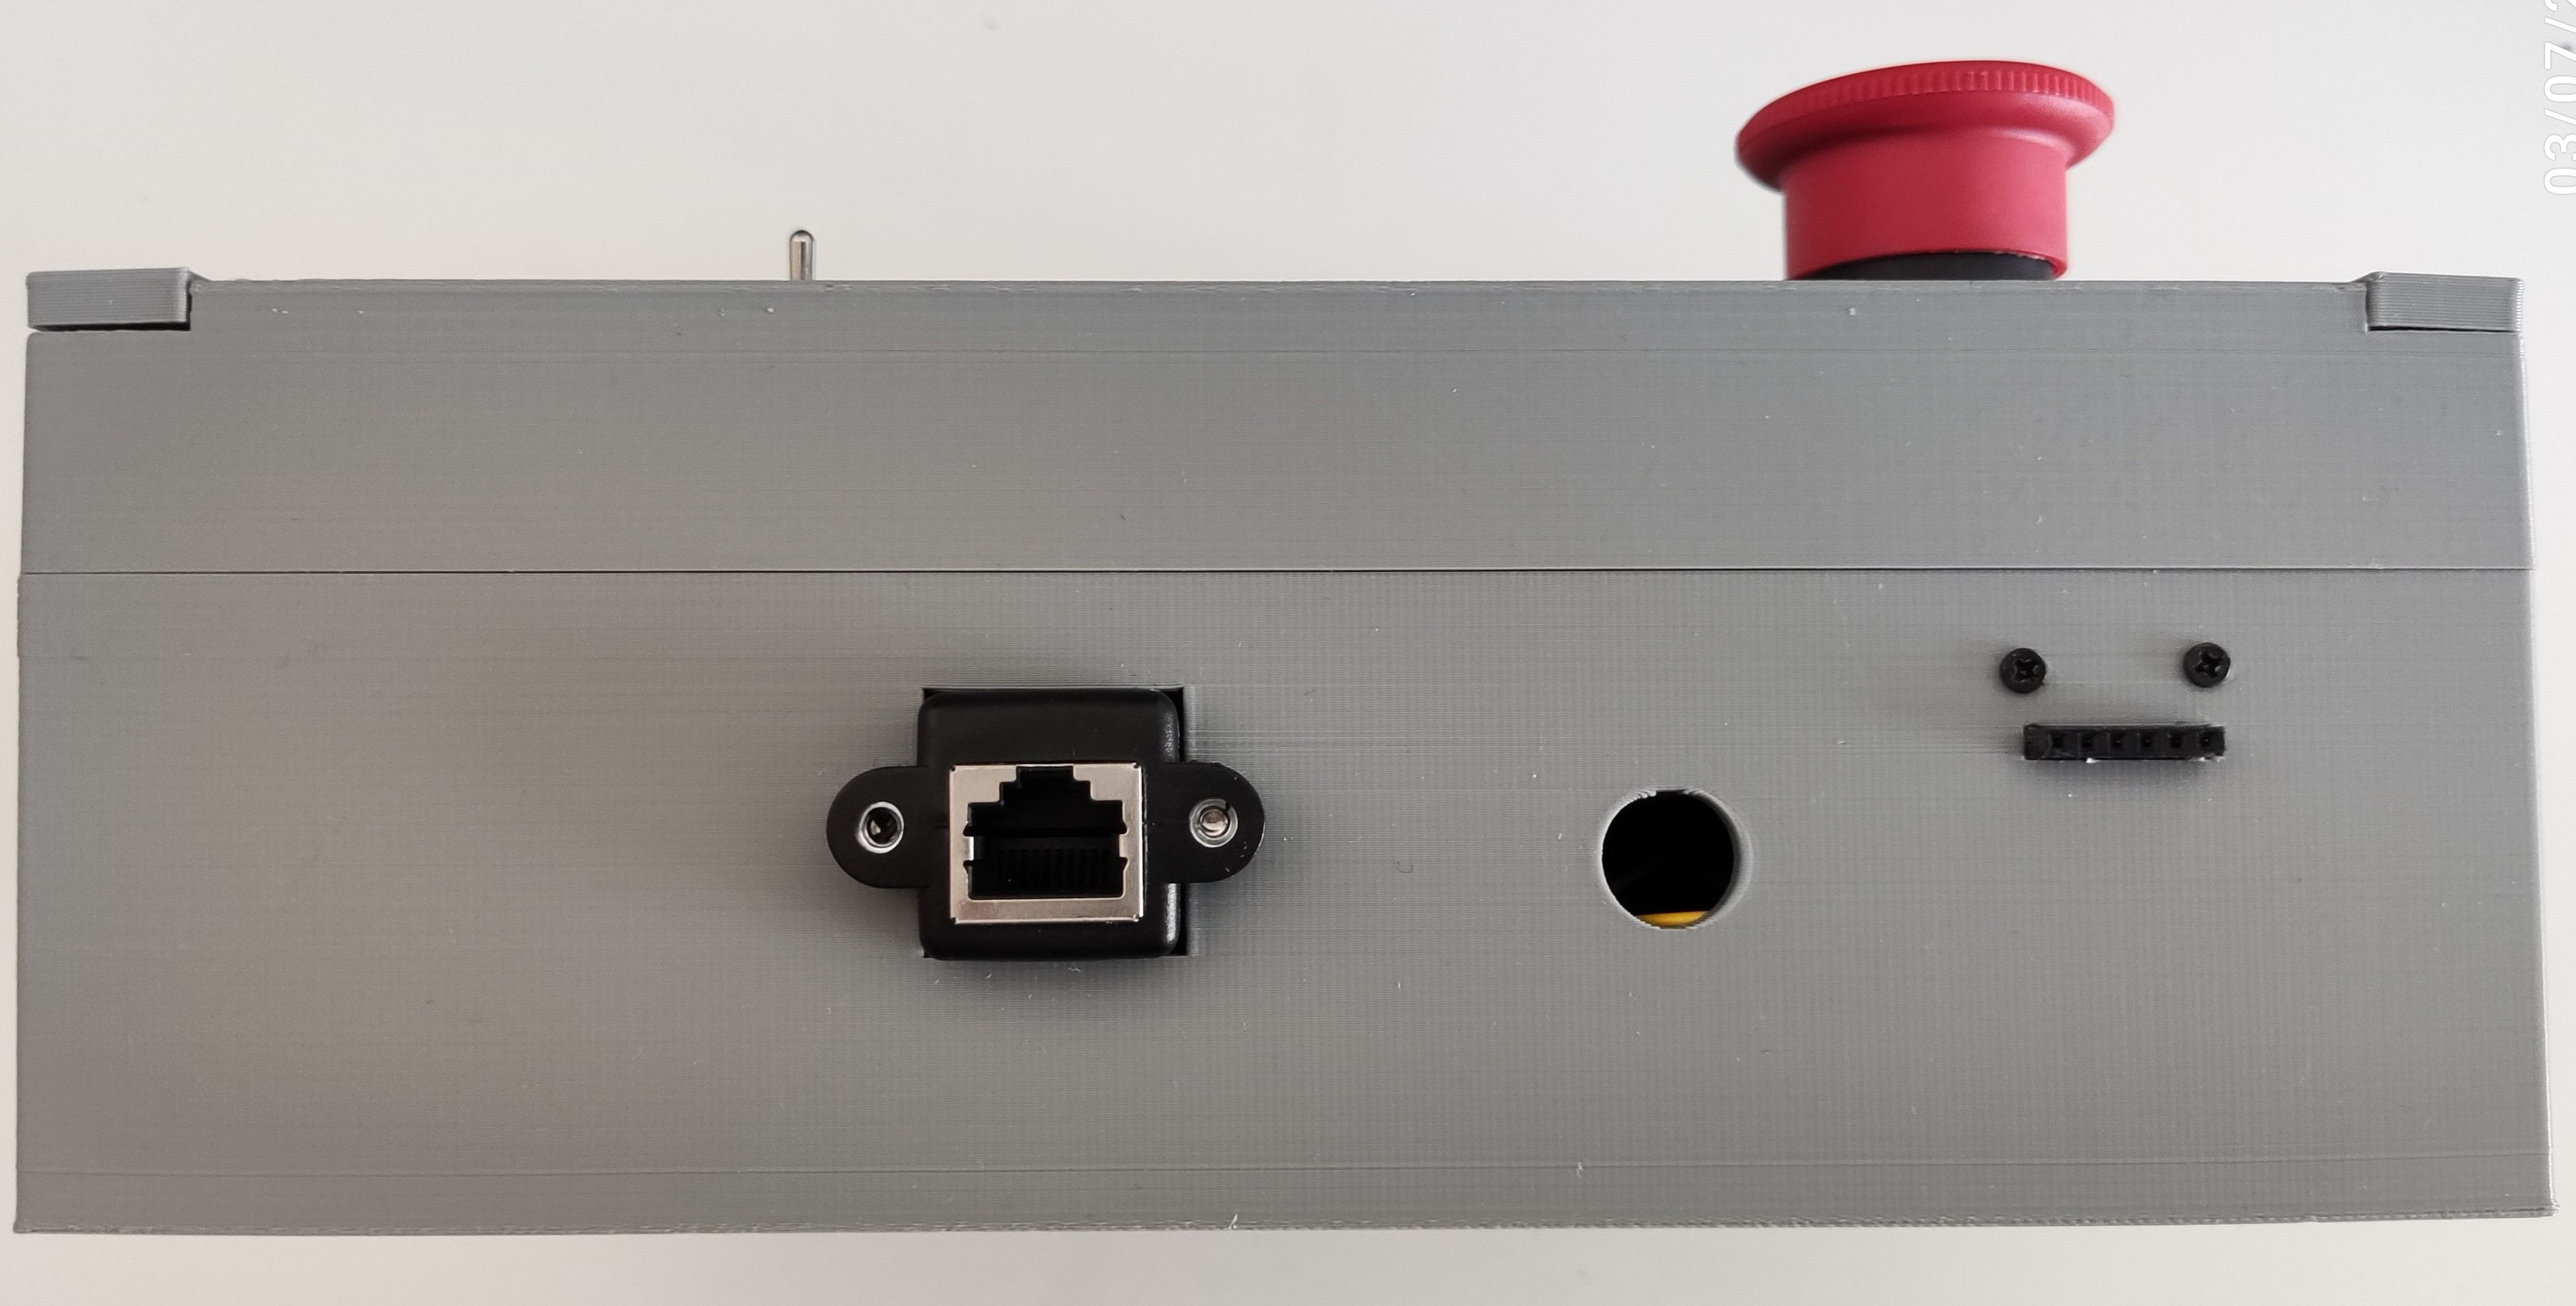
\includegraphics[width=0.75\textwidth]{07-resultados/cajatrasero.jpg}
    \caption{}
    \label{fig:cajatrasero} 
\end{figure}



\section{Integración de componentes}

Una vez fabricadas la caja en su exterior y las placas electrónicas, se integran todos 
los dispositivos y se realizan las conexiones pertinentes. En la figura \ref{fig:cajainterior}
se muestra el interior de la base de la caja, con todos los cables y conexiones internas.

\begin{figure}[hbtp]%  
    \centering 
        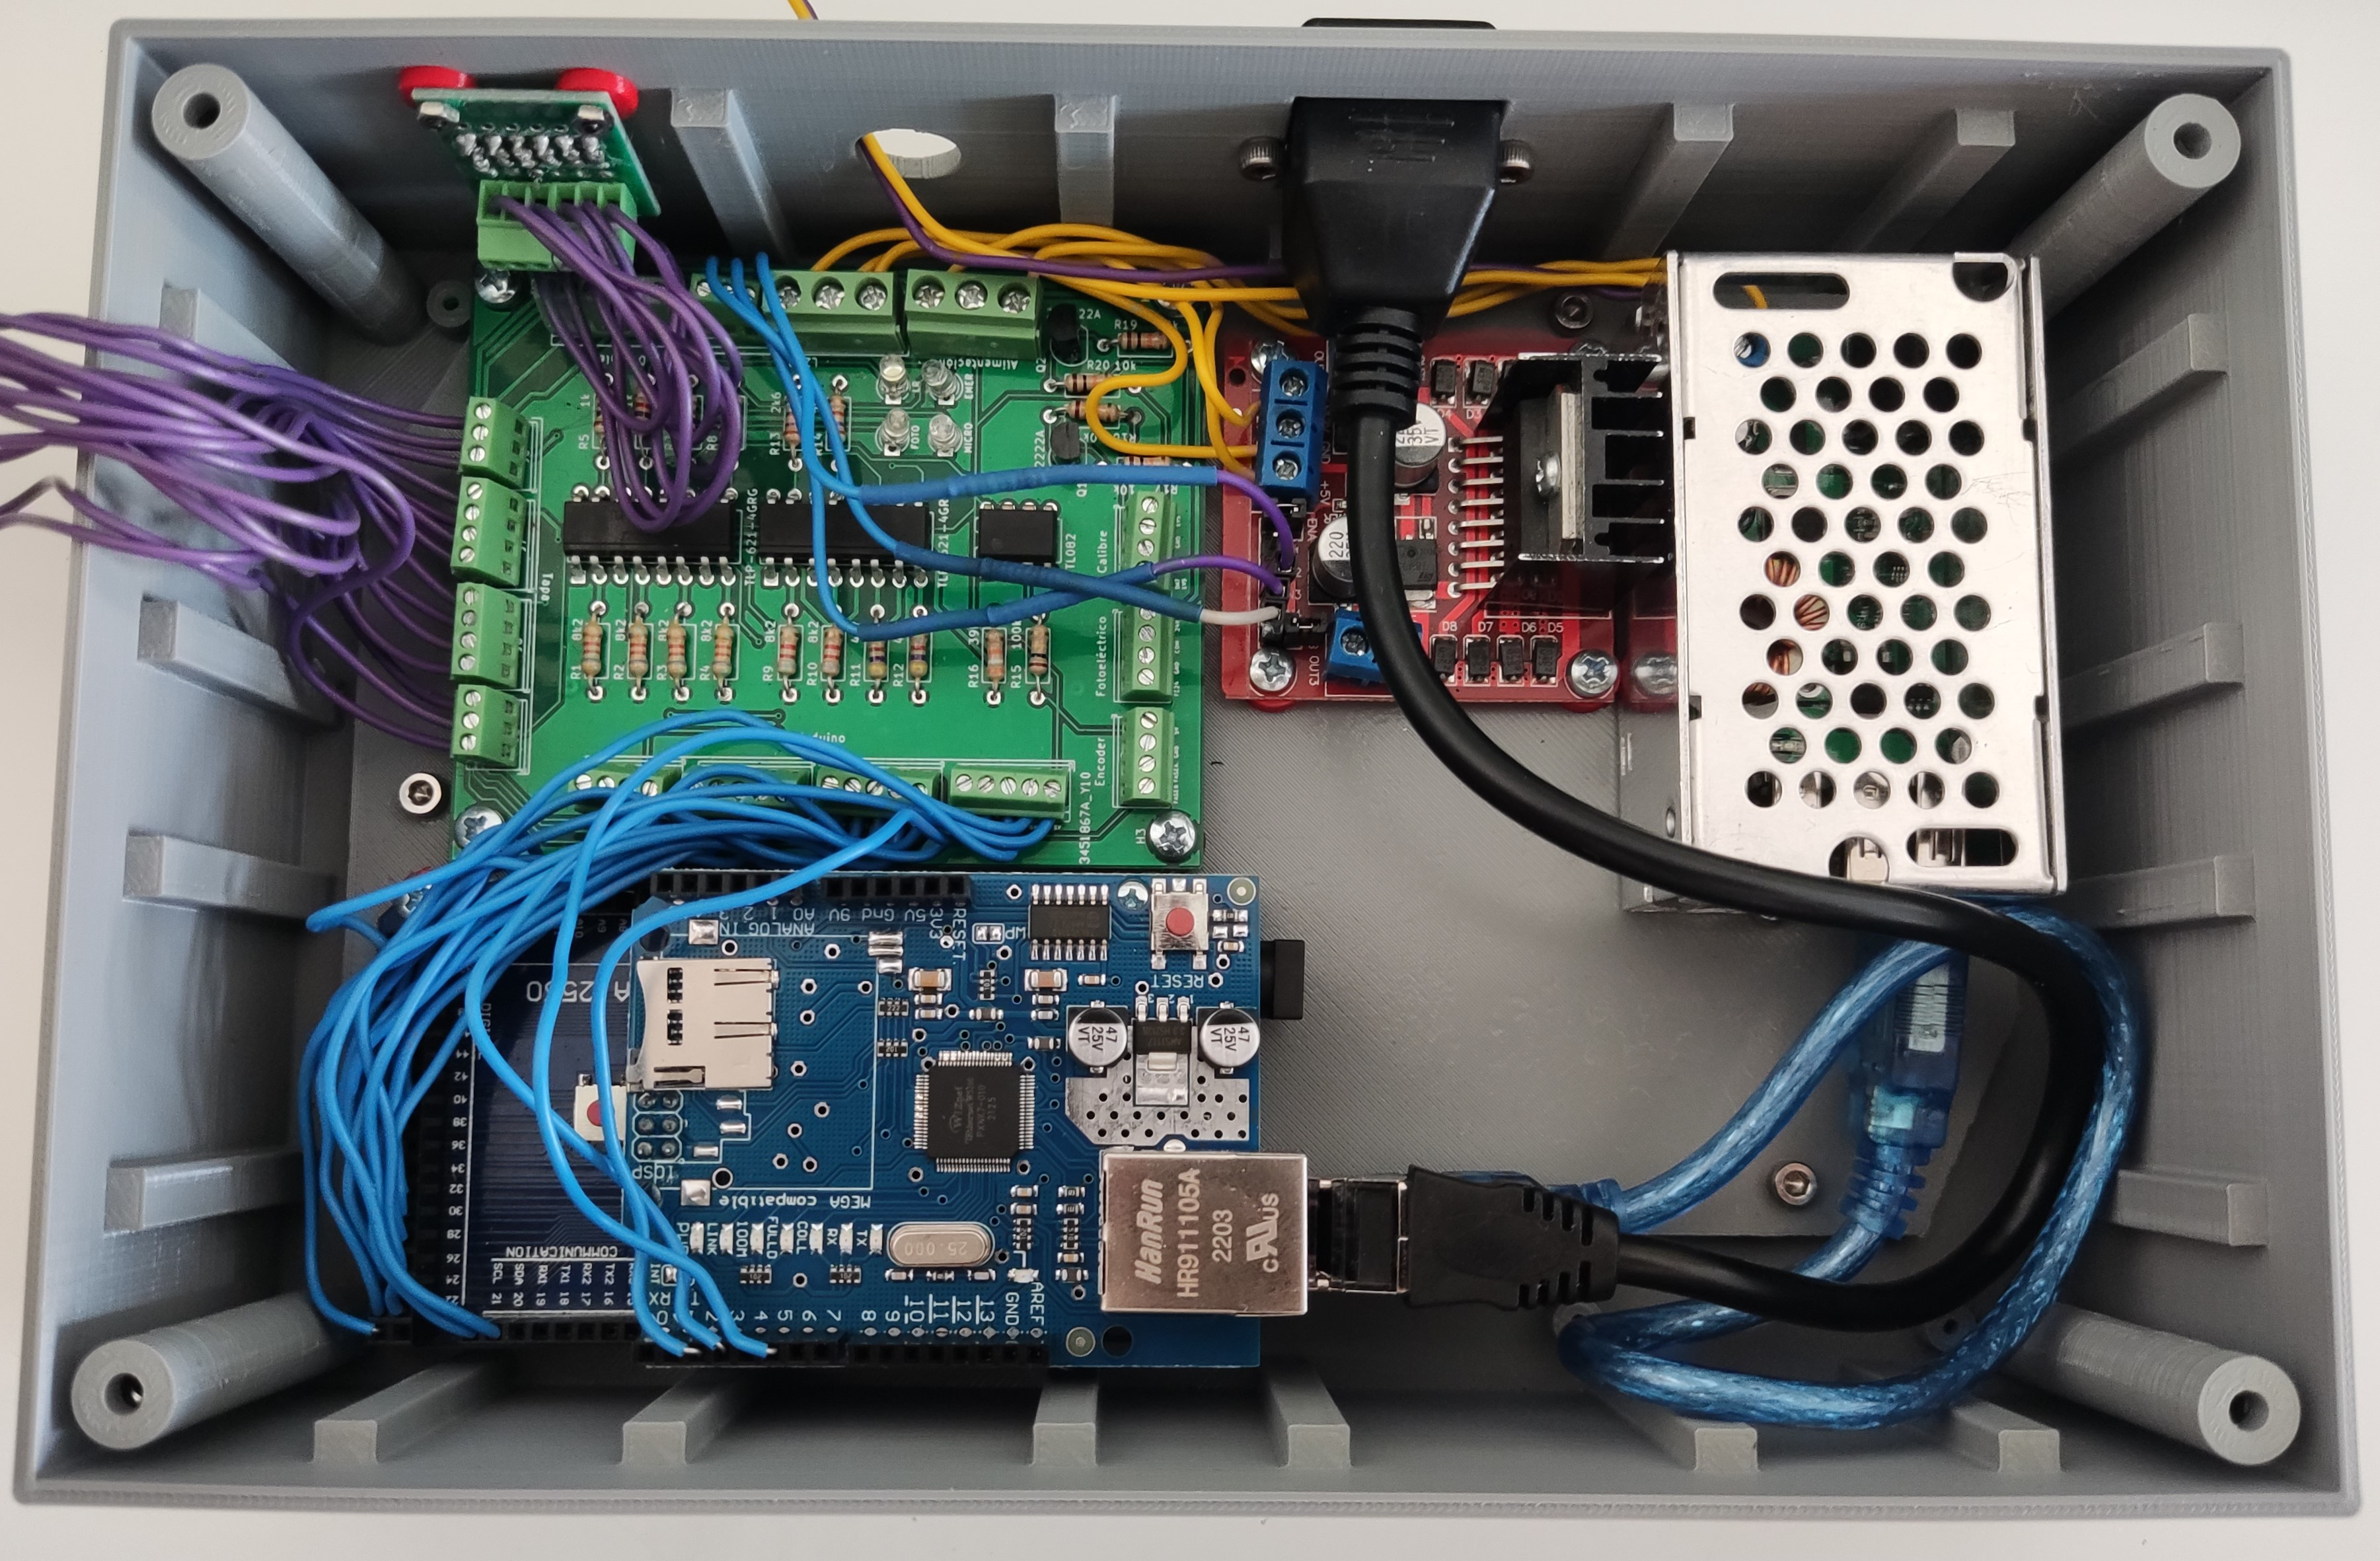
\includegraphics[width=0.75\textwidth]{07-resultados/cajainterior.jpg}
    \caption{}
    \label{fig:cajainterior} 
\end{figure}

Por otro lado, en la figura \ref{fig:cajatapainterior} se muestra el interior de la tapa de la 
caja, mostrando cómo están conectados los botones, los interruptores, la seta y el LCD.

\begin{figure}[hbtp]
    \centering 
        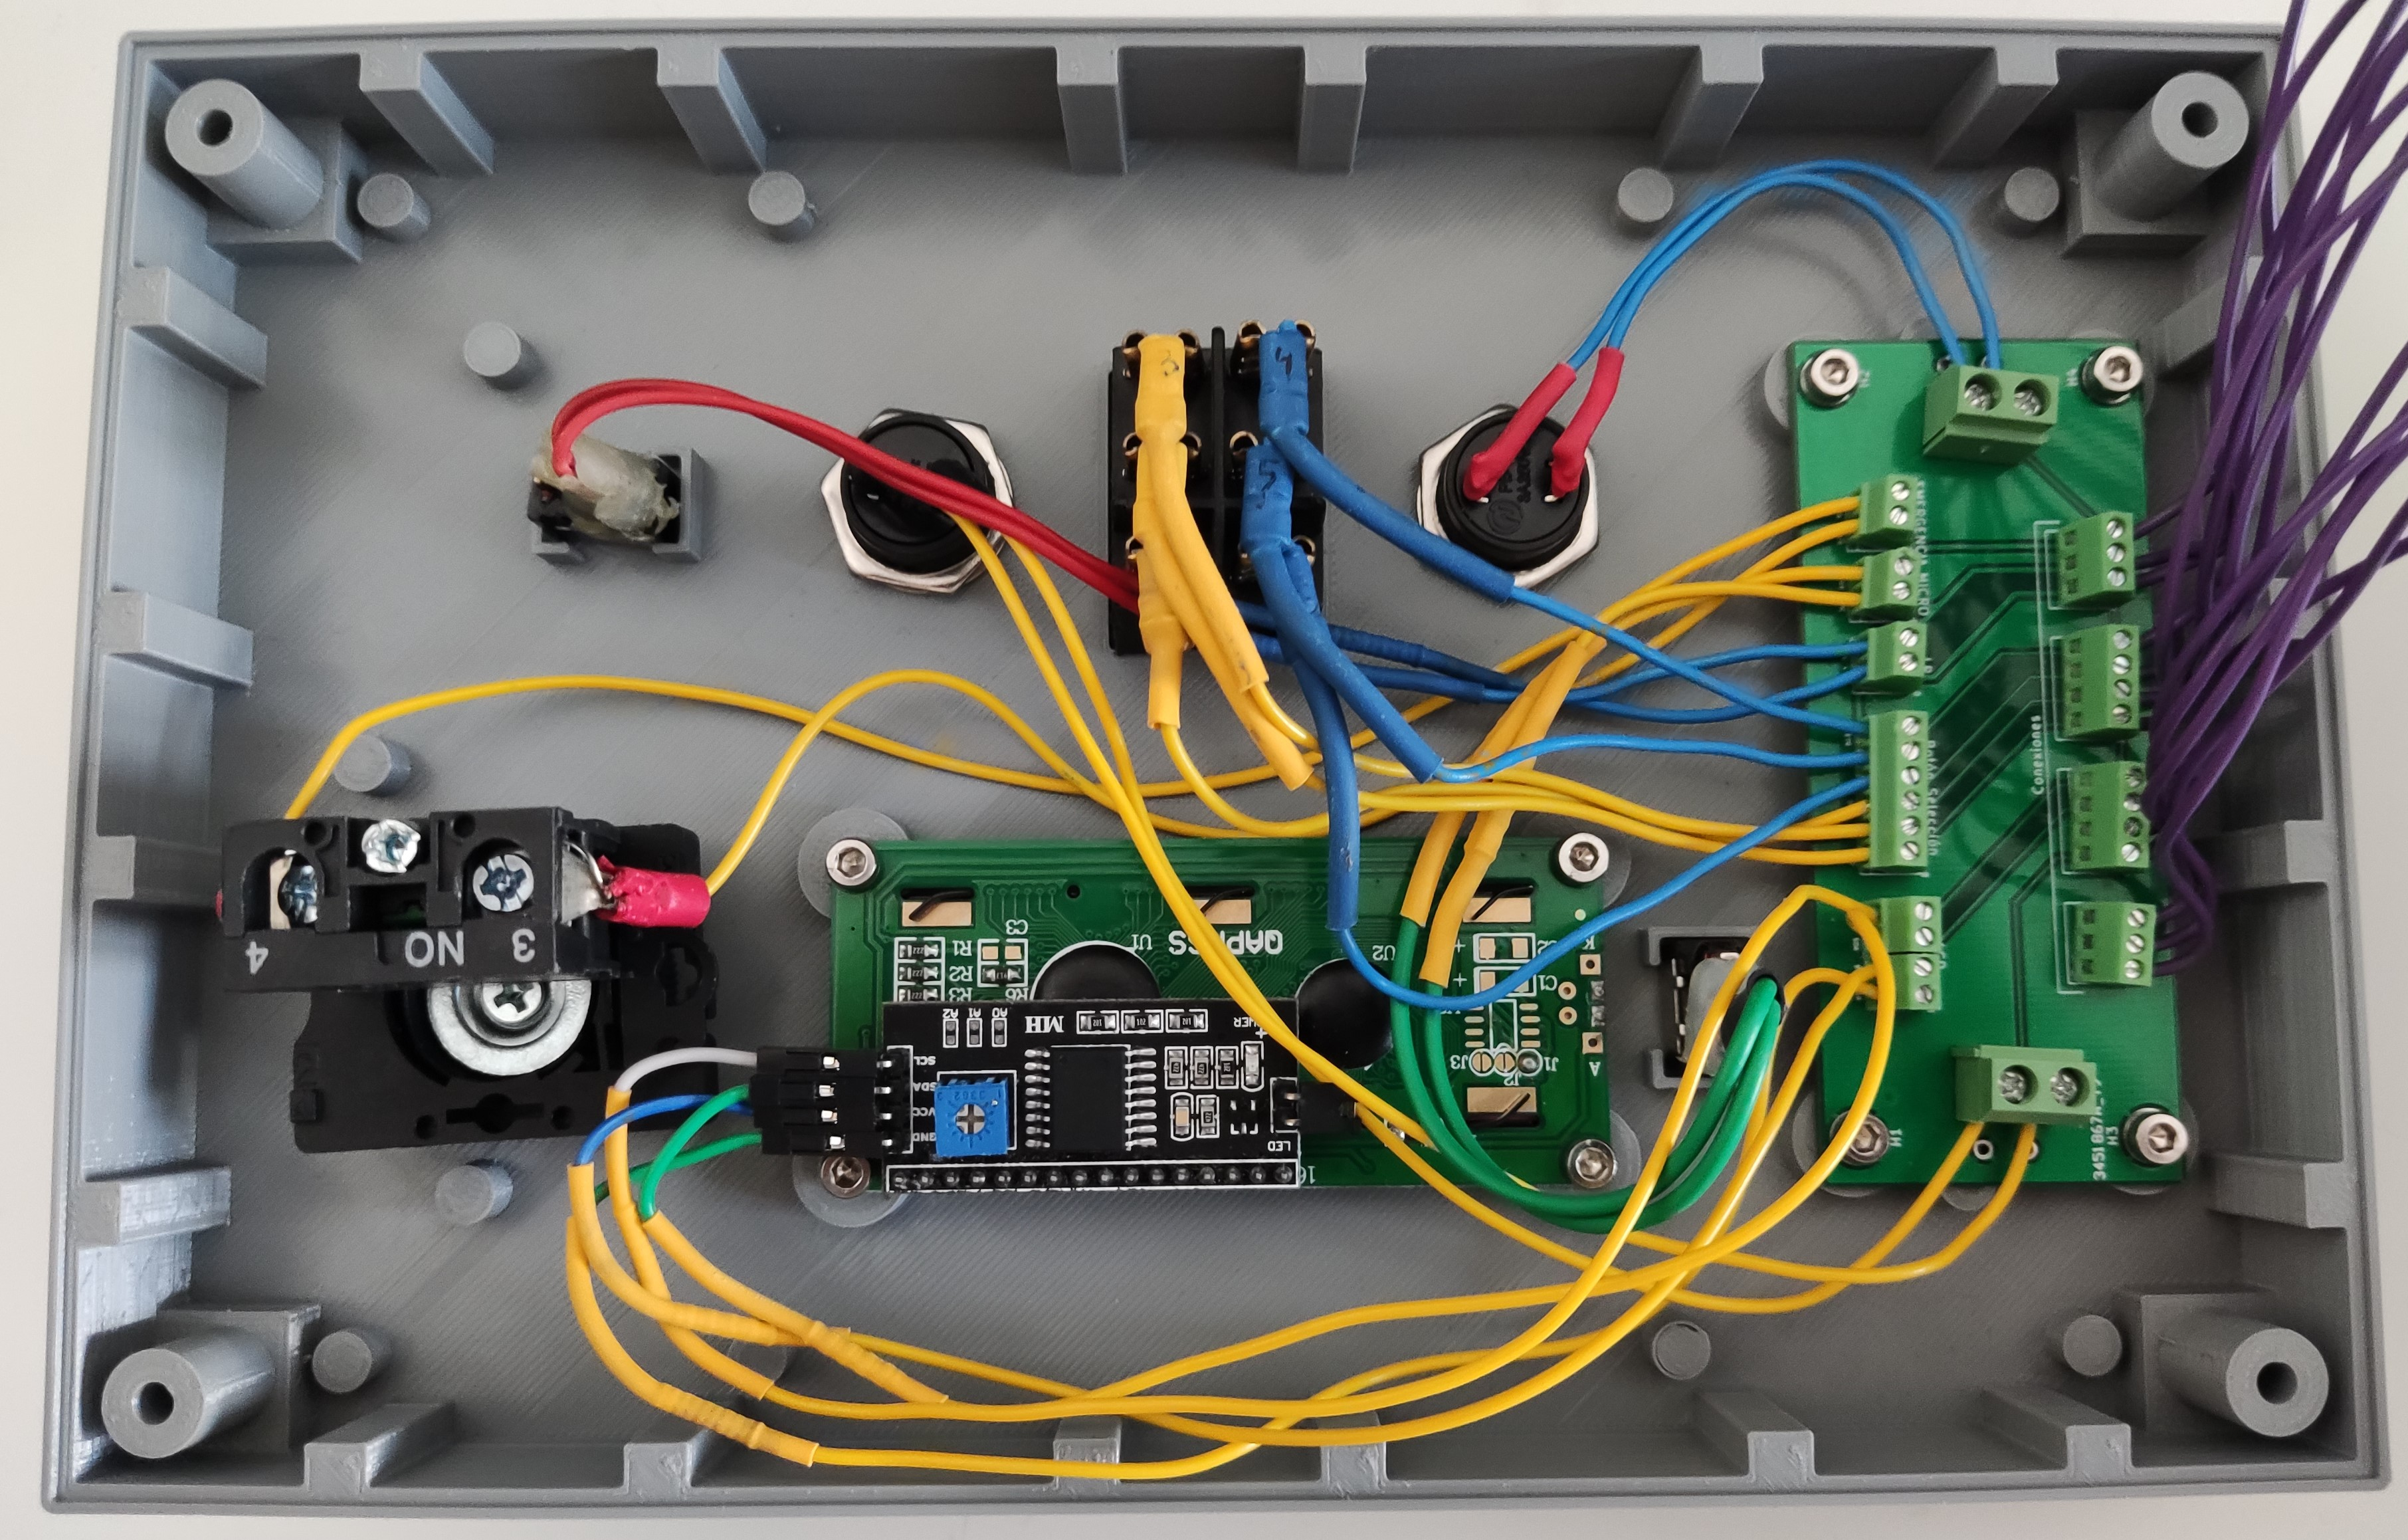
\includegraphics[width=0.75\textwidth]{07-resultados/cajatapa.jpg}
    \caption{}
    \label{fig:cajatapainterior} 
\end{figure}


\section{Modos}

Por último, se muestra el sistema encendido en sus diferentes modos en función de la posición
de las palancas y el estado de la seta de emergencia.

\begin{figure}[hbtp]%  
    \centering 
        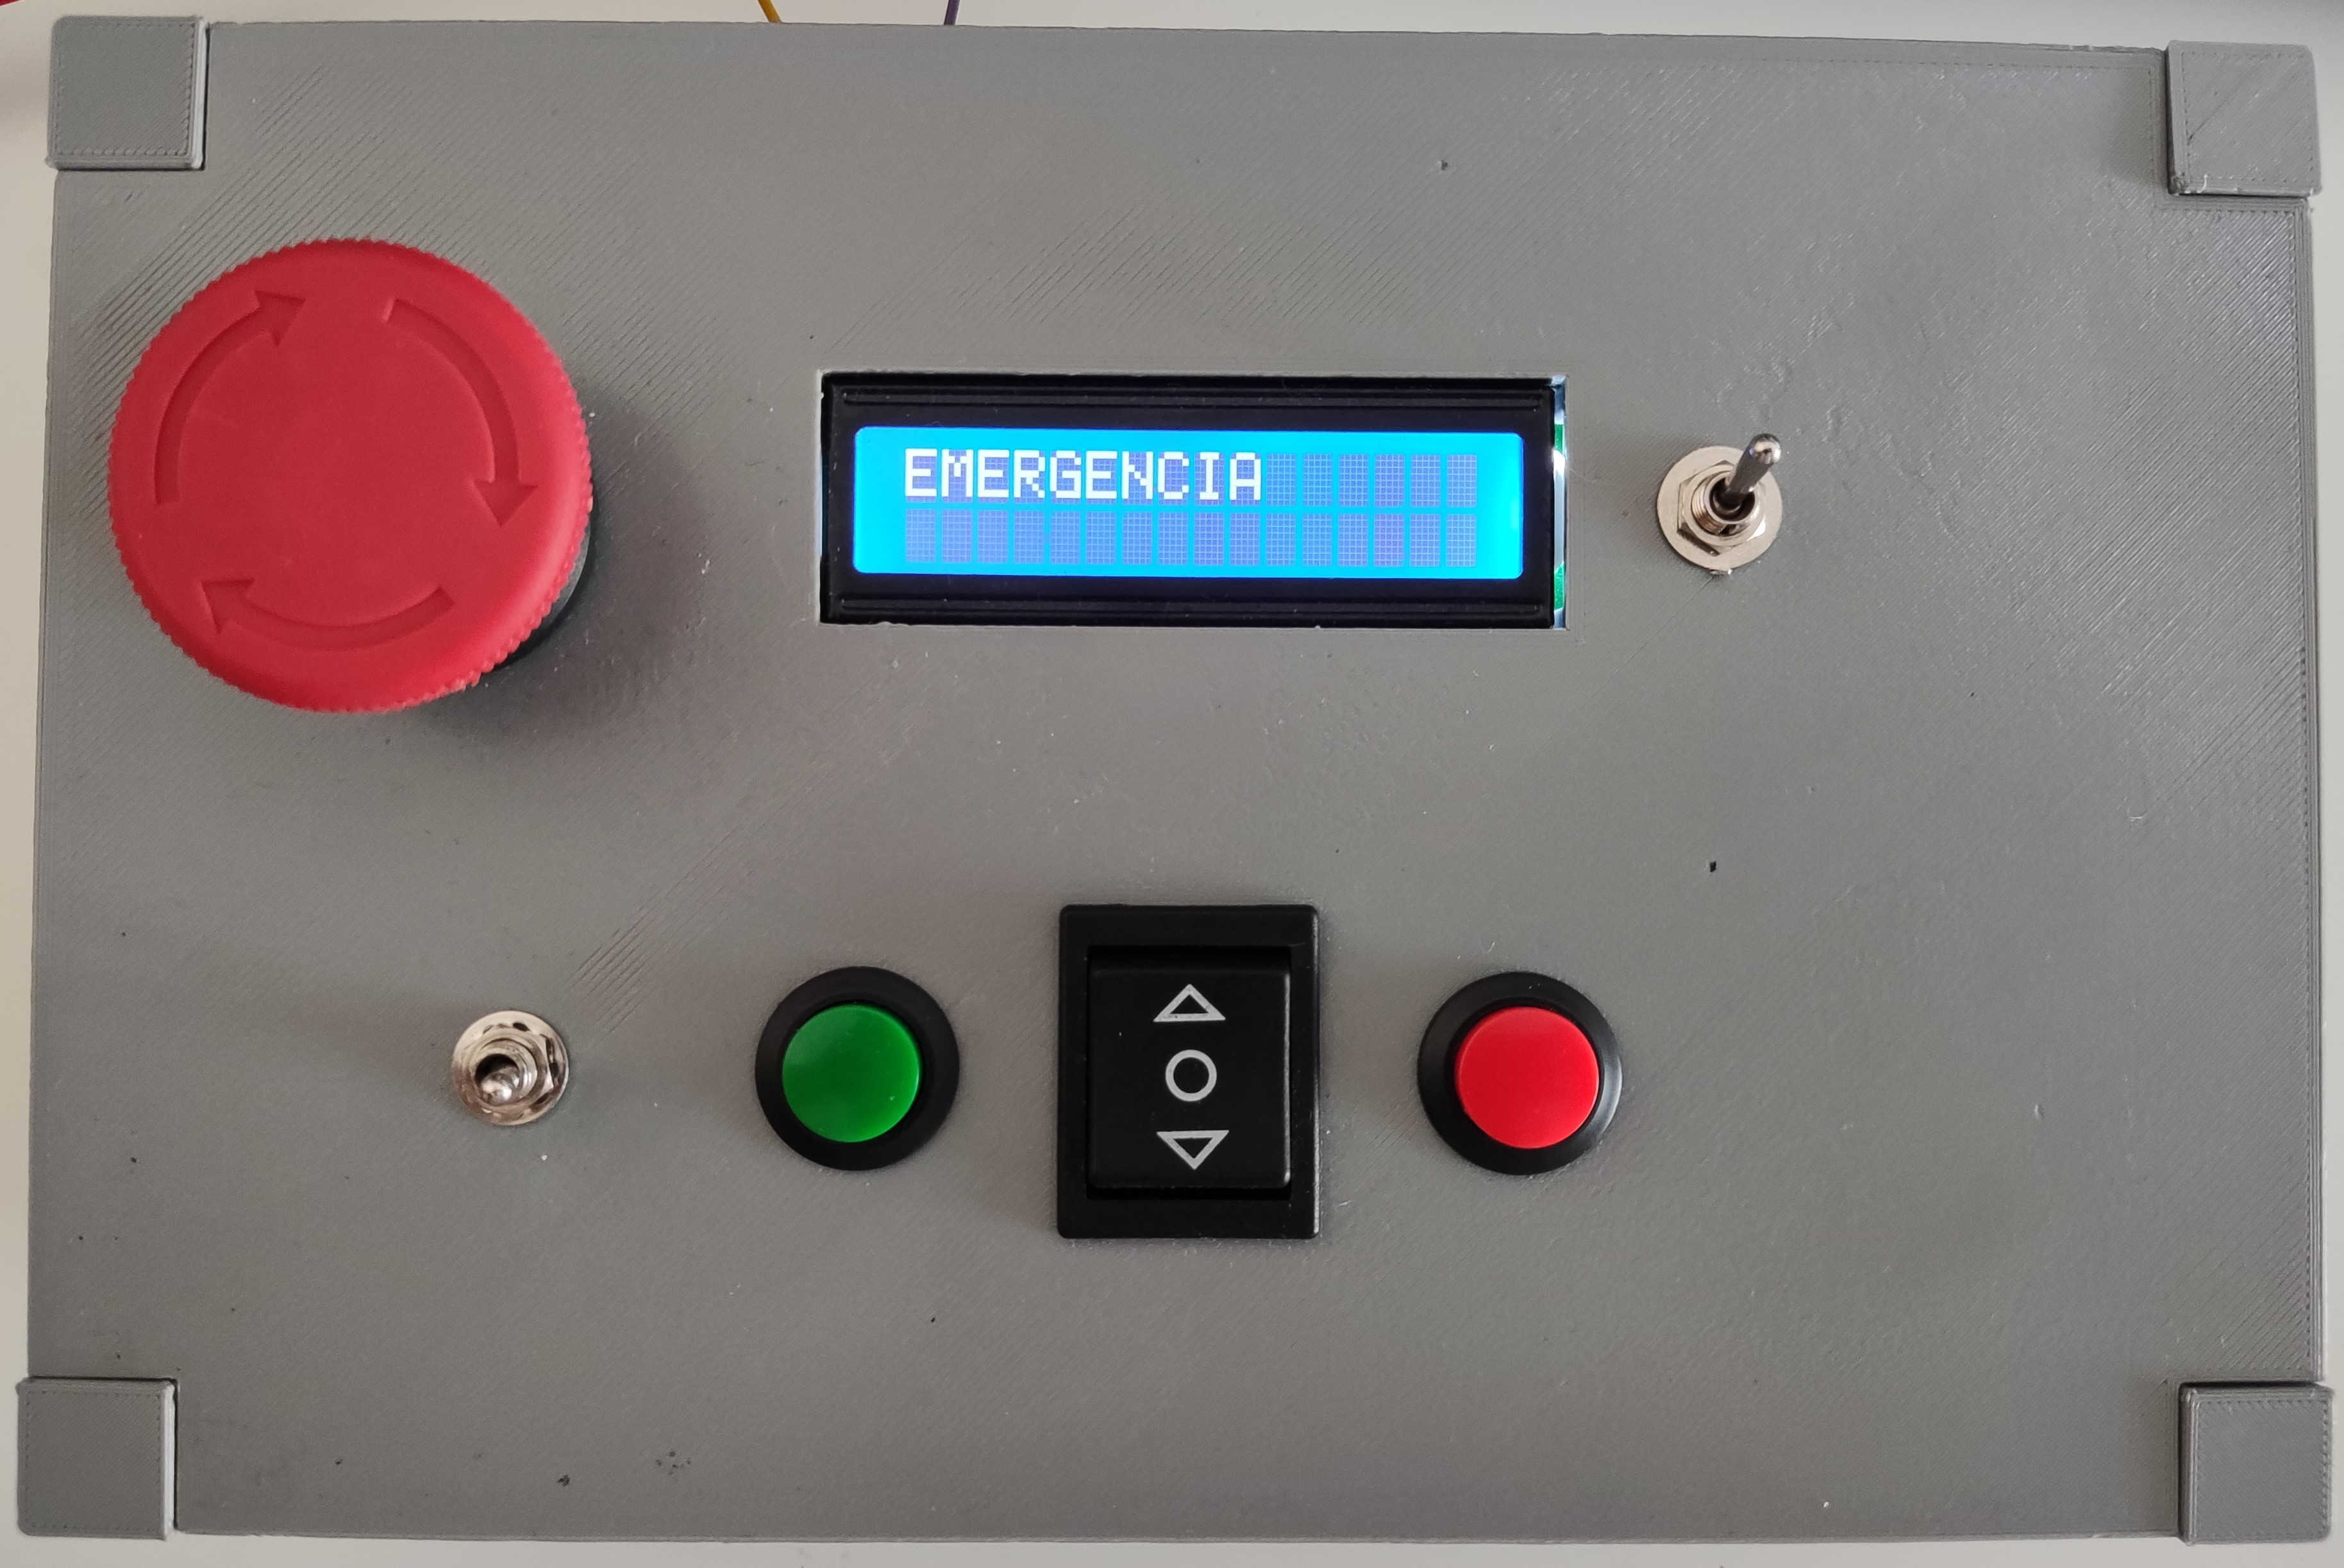
\includegraphics[width=0.75\textwidth]{07-resultados/modoemer.jpg}
    \caption{}
    \label{fig:modoemer} 
\end{figure}

\begin{figure}[hbtp]%  
    \centering 
        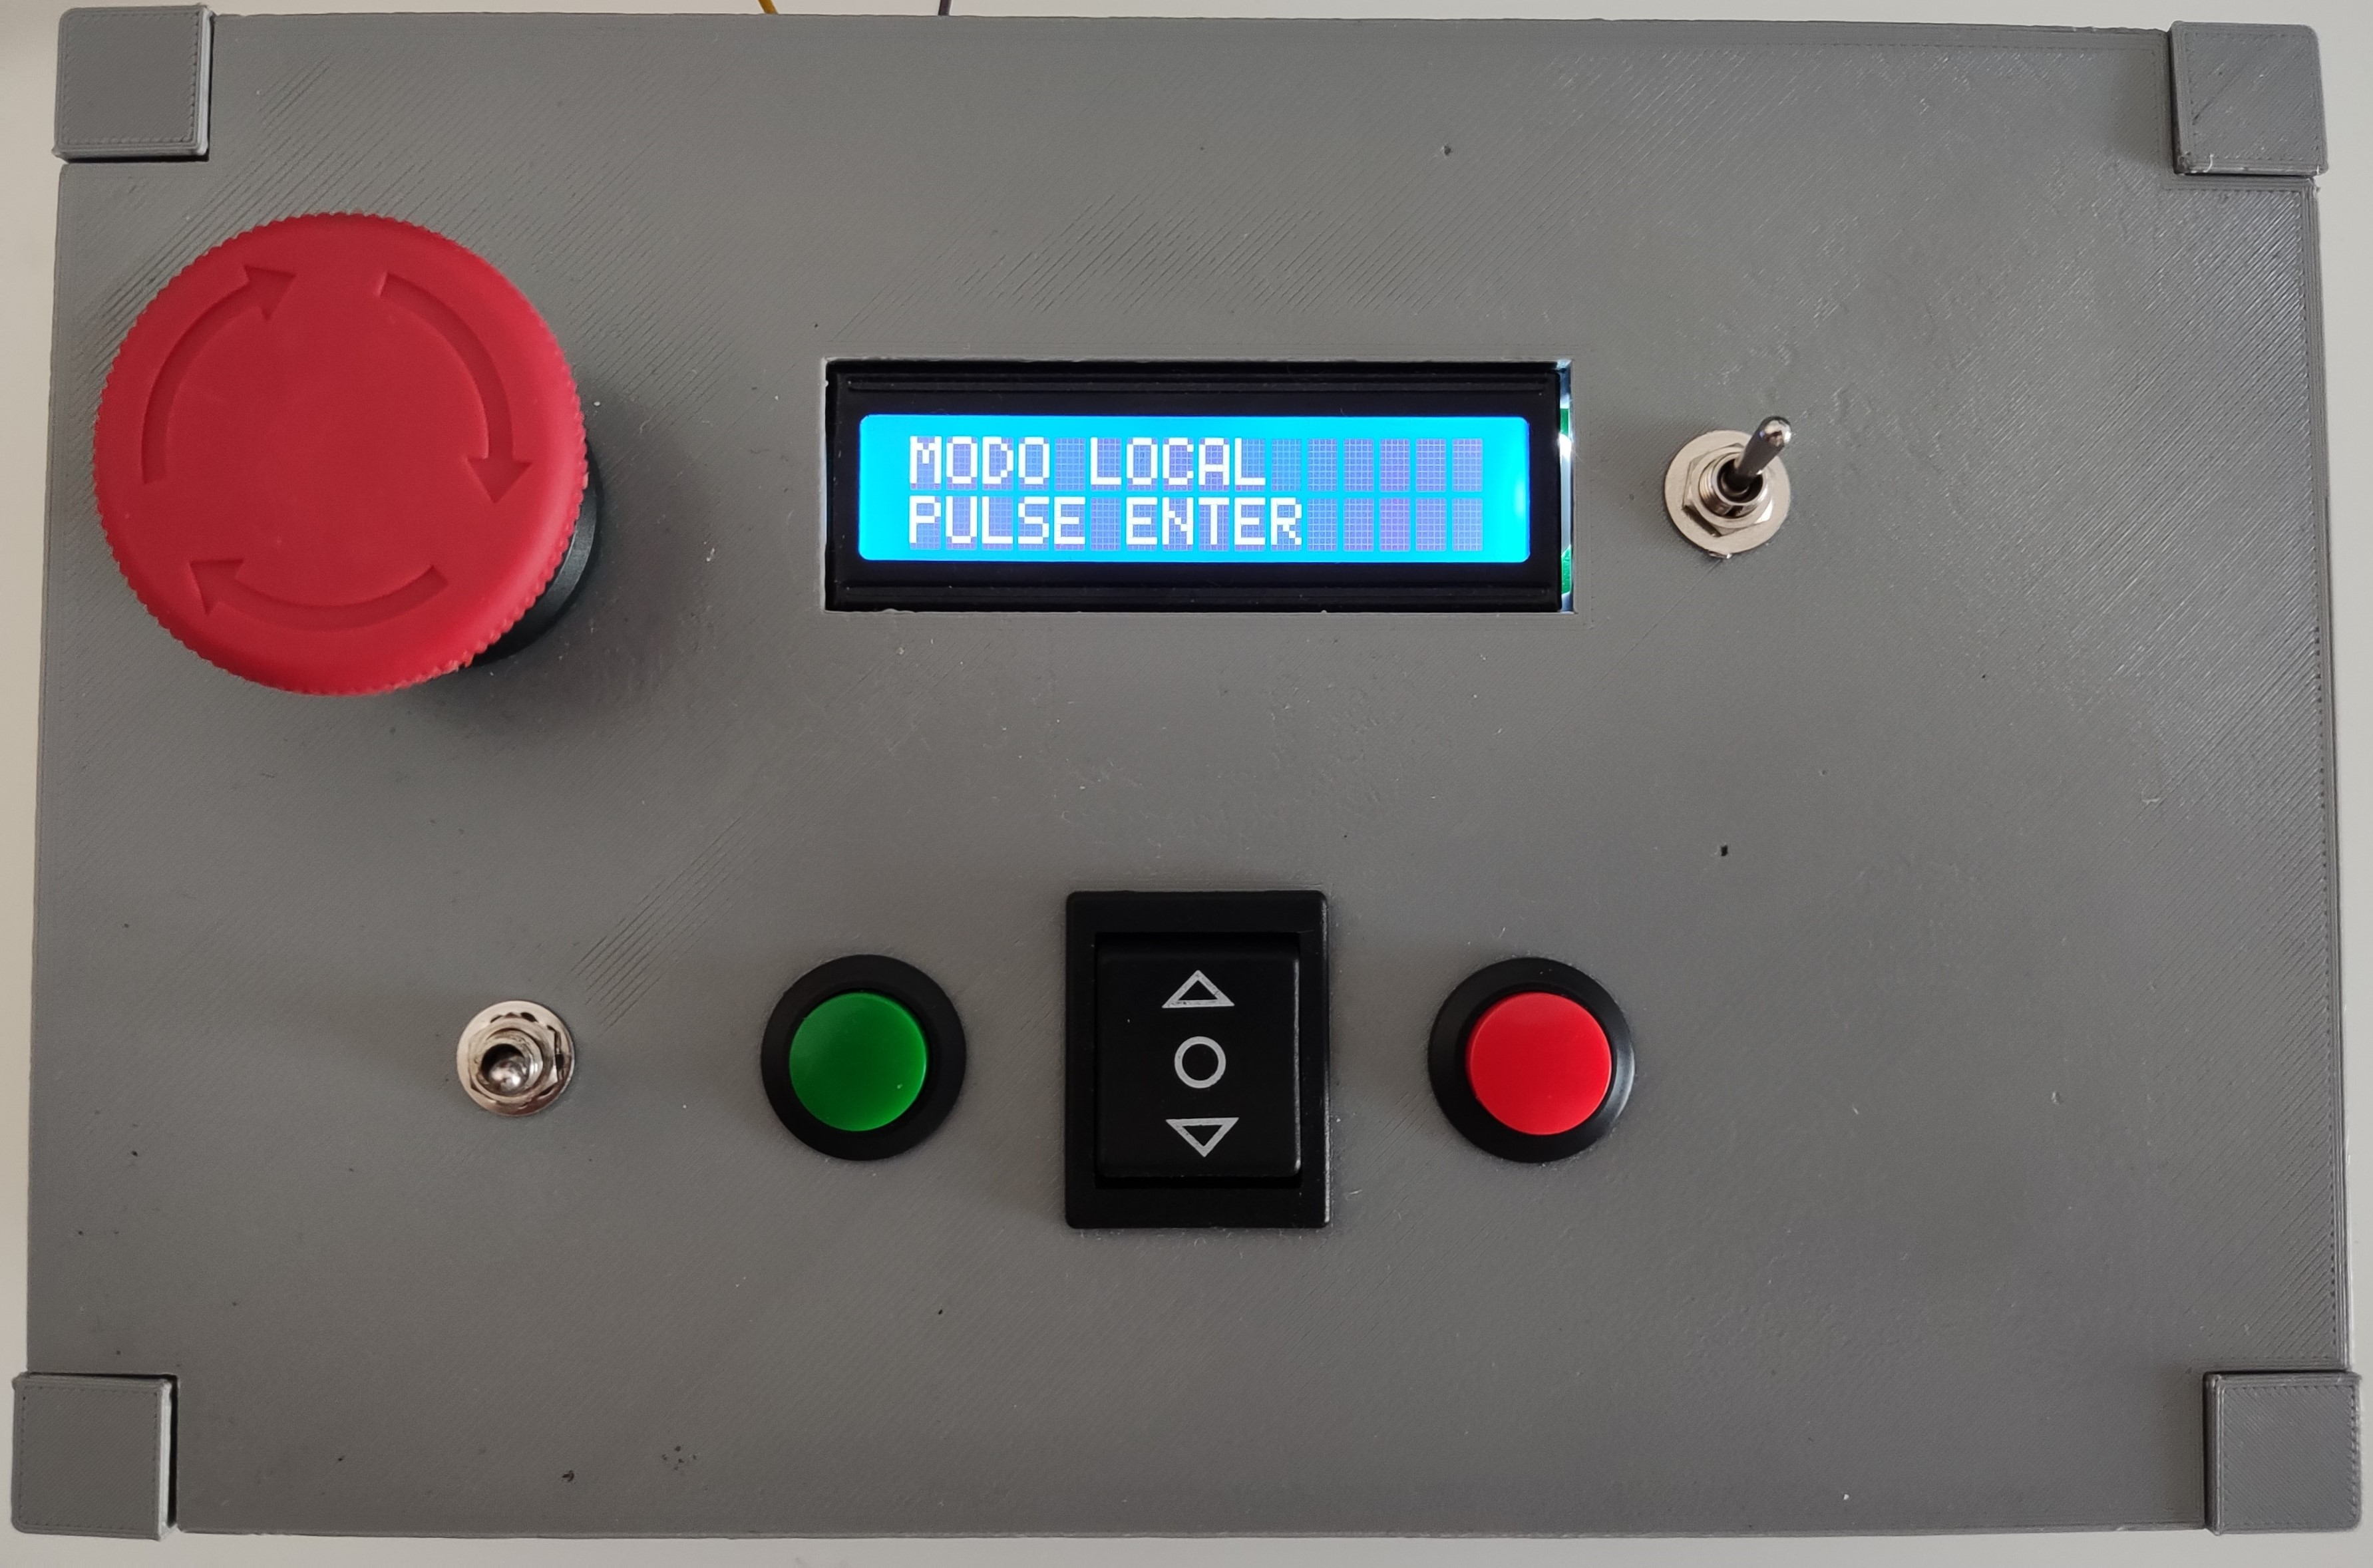
\includegraphics[width=0.75\textwidth]{07-resultados/modolocal.jpg}
    \caption{}
    \label{fig:modolocal} 
\end{figure}

\begin{figure}[hbtp]%  
    \centering 
        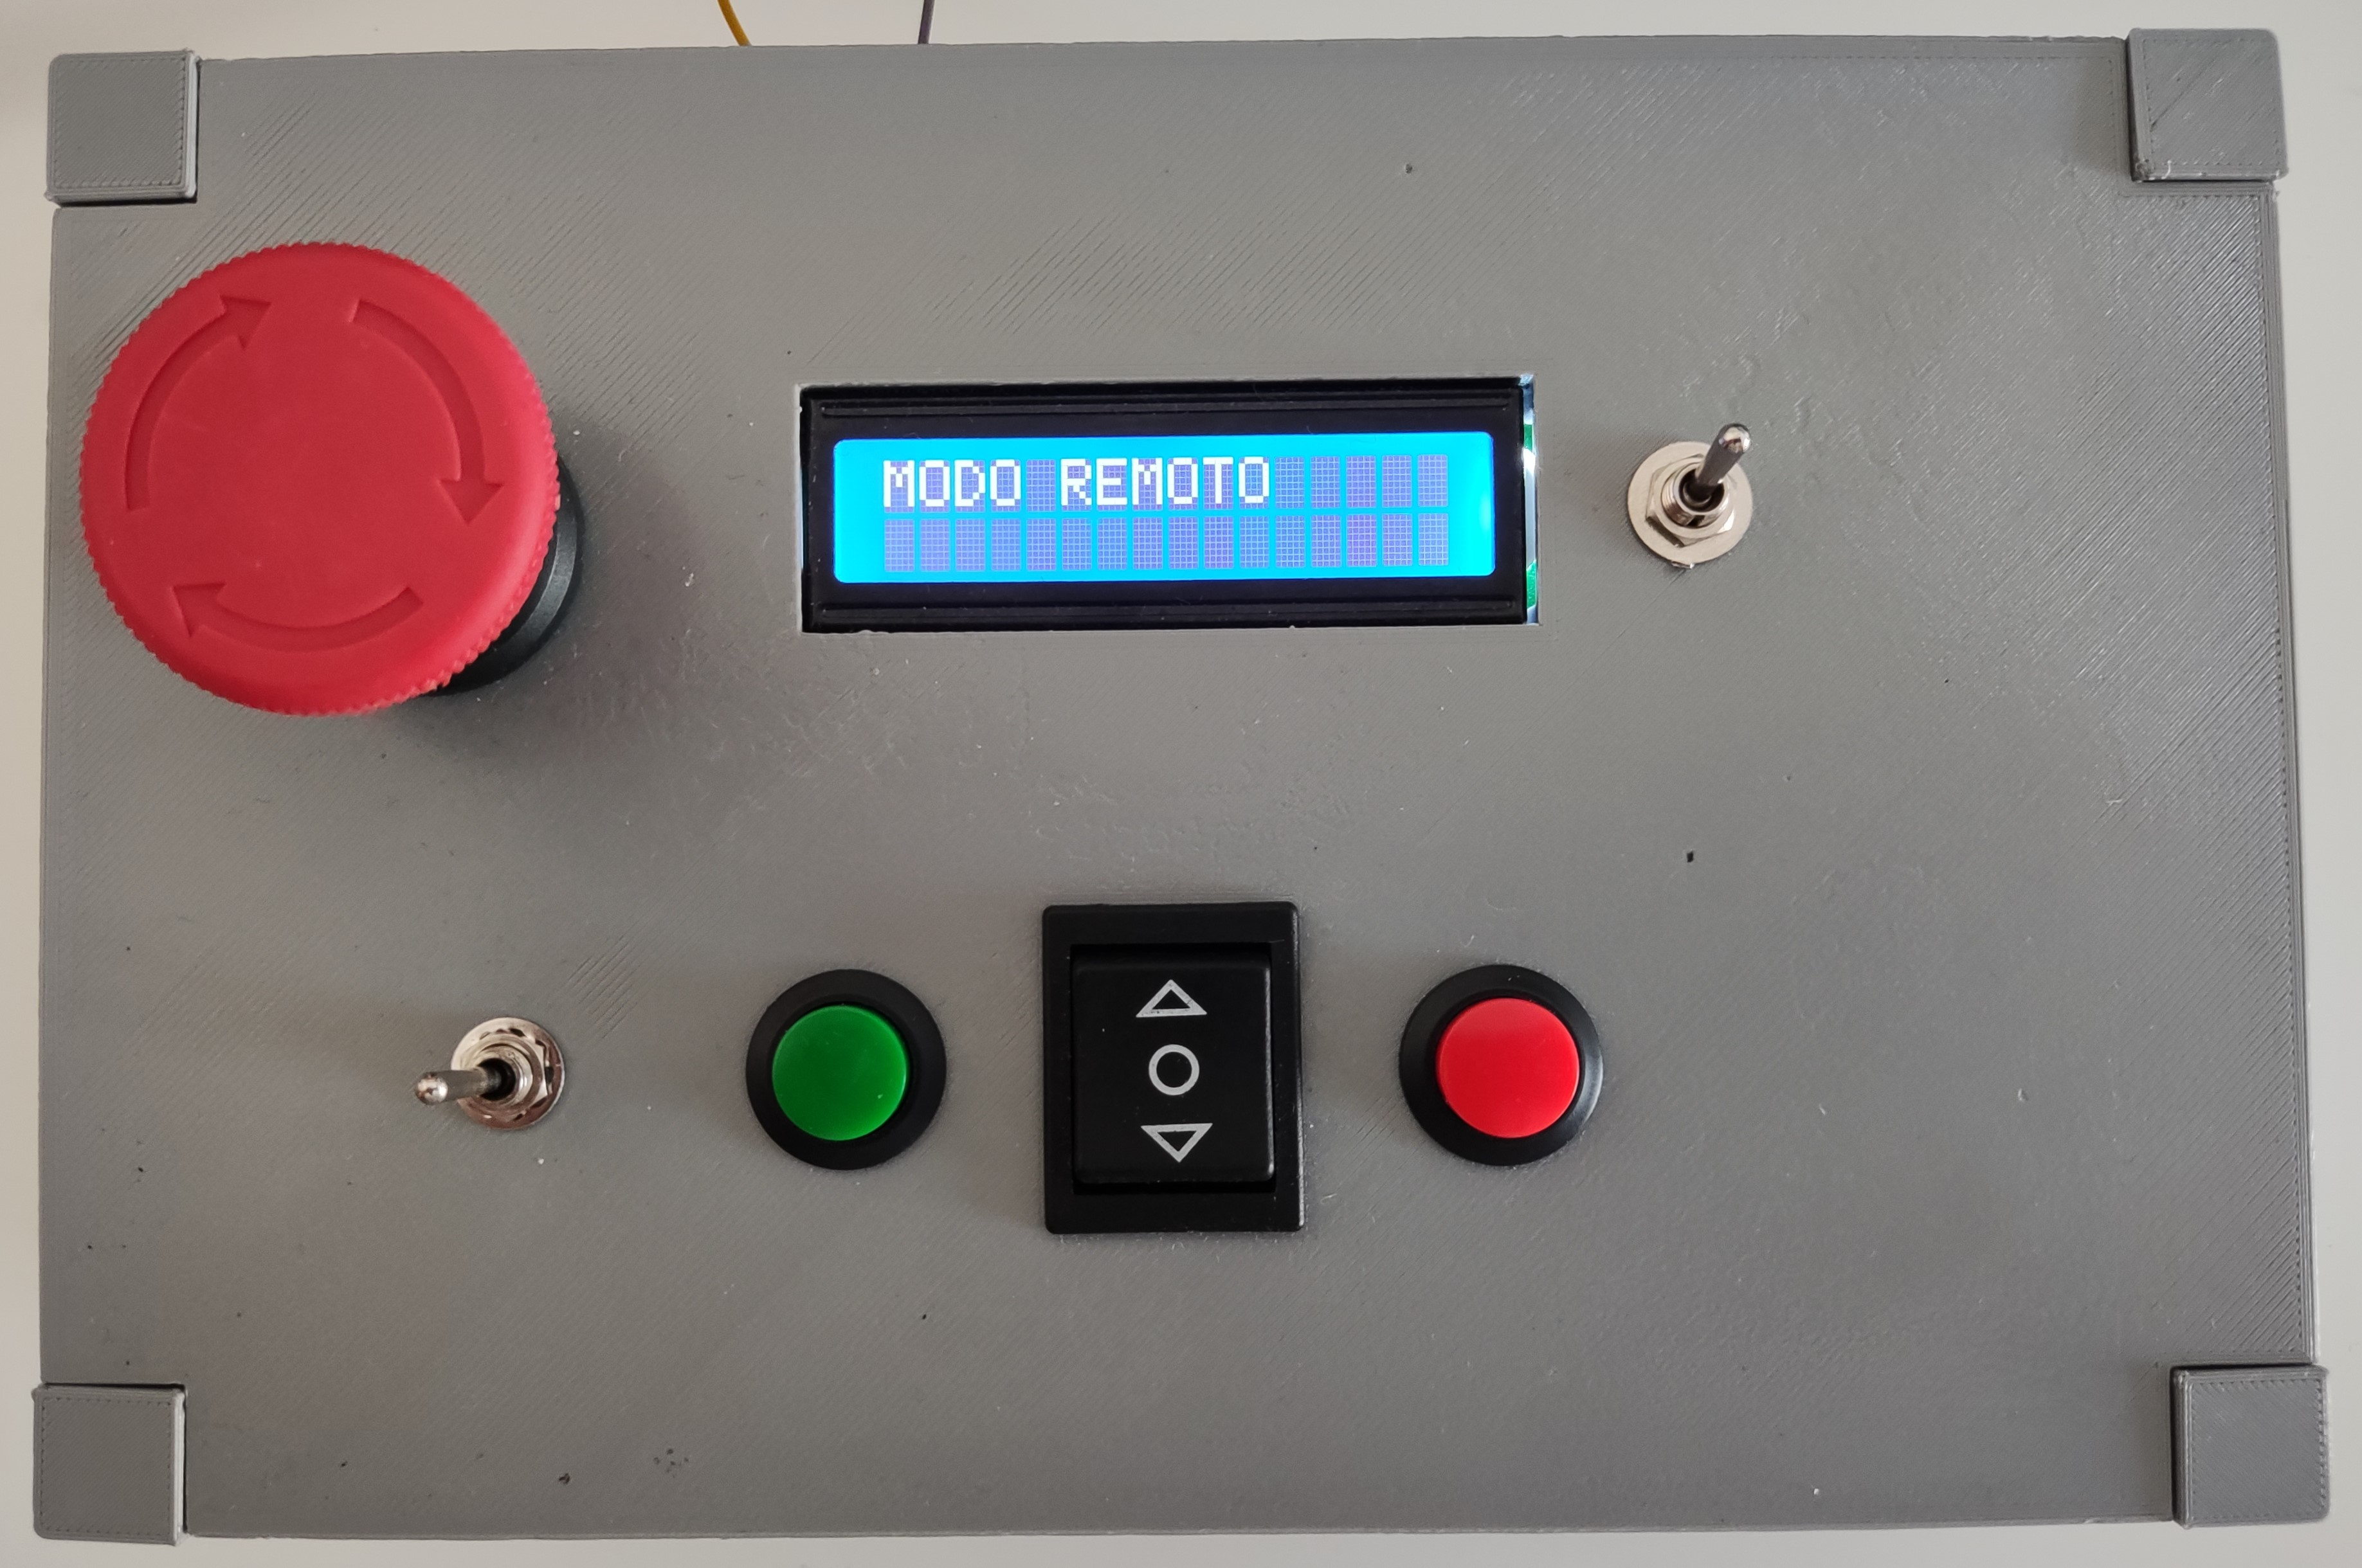
\includegraphics[width=0.75\textwidth]{07-resultados/modoremoto.jpg}
    \caption{}
    \label{fig:modoremoto}
\end{figure}

\begin{figure}[hbtp]%  
    \centering 
        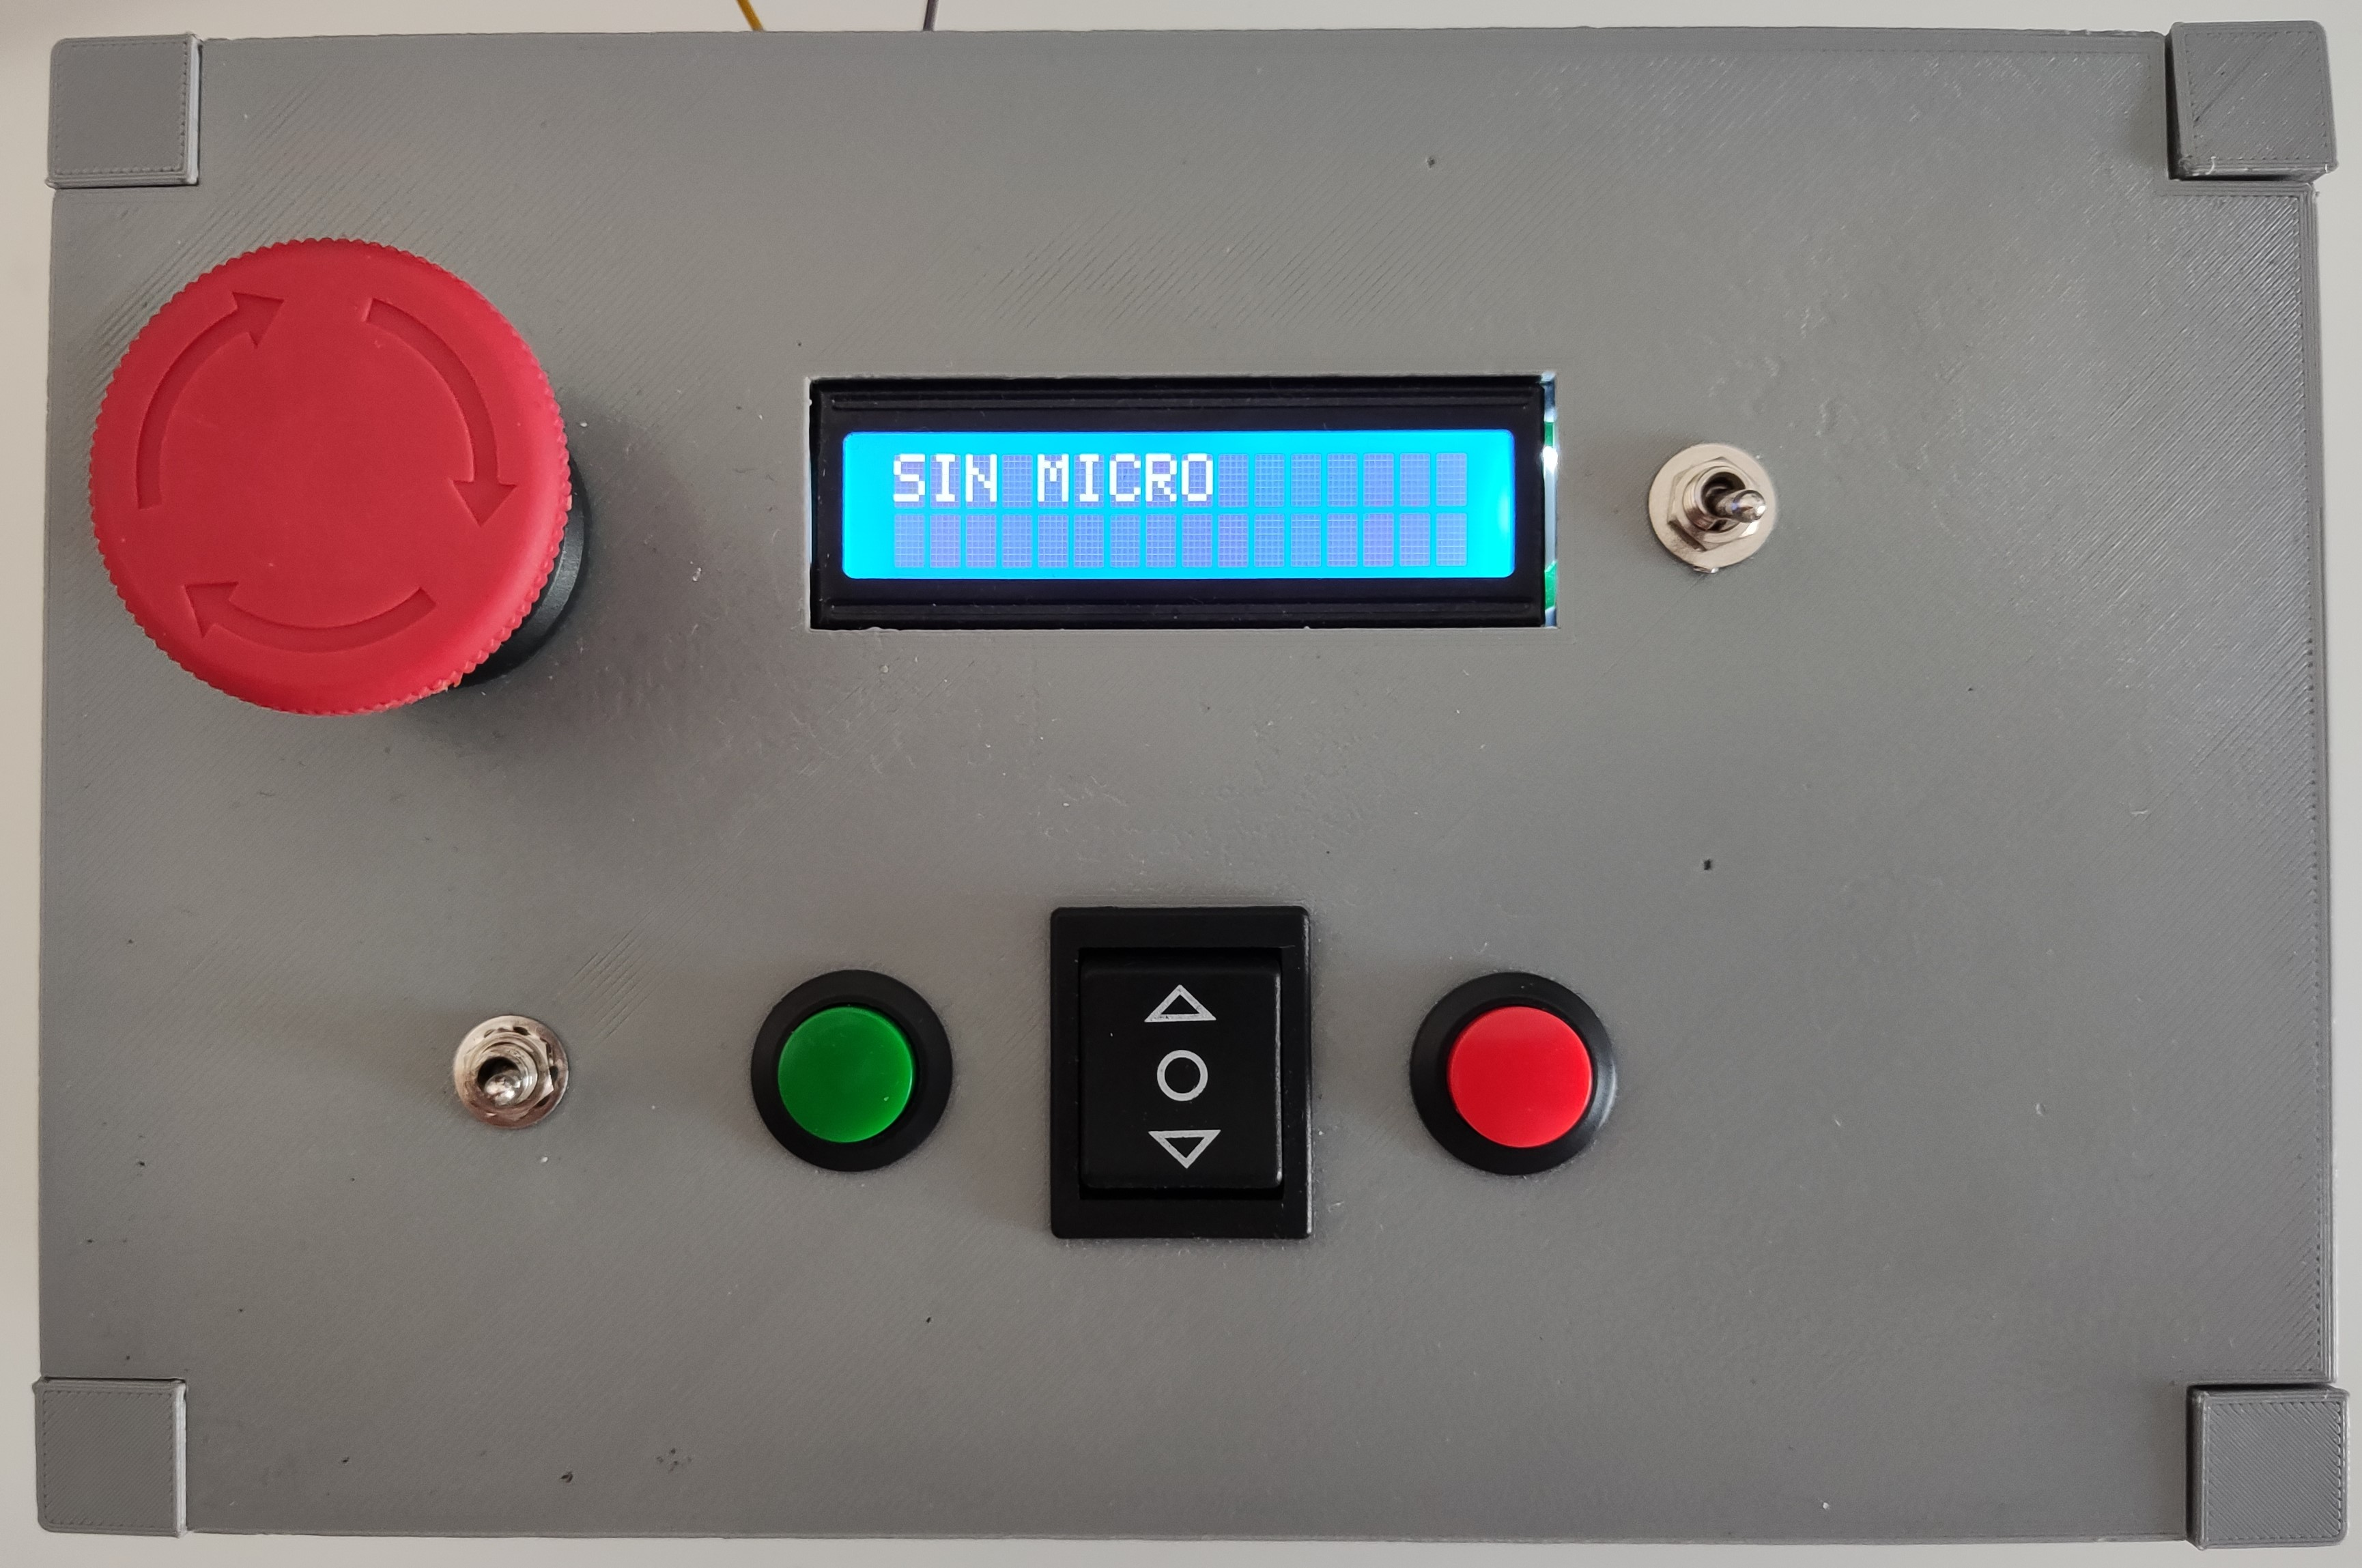
\includegraphics[width=0.75\textwidth]{07-resultados/modosinmicro.jpg}
    \caption{}
    \label{fig:modosinmicro} 
\end{figure}
